\chapter{\label{ch:5-qd-result}Application to simulated and real phenotypes in UK Biobank}

\minitoc

\section{Chapter overview}

In this chapter we apply Quickdraws to simulated and real phenotypes in the UK Biobank \cite{bycroft2018uk}. We start by discussing data and quality control steps we used to perform GWAS in the UK Biobank in Section \ref{sec:ch5-data}. In order to assess the calibration and demonstrate statistical power we then perform simulation studies in Section \ref{sec:ch5-sim} across a wide variety of designs varying relatedness, population structure, prevalence and the genetic architecture of the simulated trait. Subsequently in Section \ref{sec:ch5-ukb}, we apply Quickdraws on 79 quantitative and 50 self-reported disease phenotypes from UK Biobank where we show Quickdraws leads to state-of-the-art statistical power while controlling for false positives. We perform a replication analysis with summary statistics from external biobanks like Biobank Japan and Finngen, followed by predictive power analysis and comparing with PGS methods. Finally in Section \ref{sec:ch5-cost}, we perform a thorough cost analysis on UK Biobank's cloud platform comparing Quickdraws against recent scalable methods like FastGWA and REGENIE. We conclude the chapter with discussing the key findings and directions for future work.

\section{Data and quality control}
\label{sec:ch5-data}

\subsection{UK Biobank data}

We used the UK Biobank SNP array data for $405{,}088$ white British samples \cite{bycroft2018uk} (in PLINK bed format \cite{purcell2007plink,chang2015second}) for model fitting and HRC+UK10k-imputed data \cite{haplotype2016reference,uk10k2015uk10k,bycroft2018uk} (in bgen v1.2 format \cite{band2018bgen}) for association testing.
%
We filtered the set of available autosomal variants to have minor allele frequency (MAF) $\geq 1\%$, Hardy-Weinberg equilibrium $p \geq 1 \times 10^{-15}$, and a genotyping rate above $99\%$, obtaining a set of $458{,}620$ markers.
%
We used these markers as input for the model-fitting step of BOLT-LMM, REGENIE, and Quickdraws, while for SAIGE we performed LD pruning using PLINK (v1.9 \cite{purcell2007plink,chang2015second} setting \texttt{--window\_size} to $50$kb, \texttt{--step\_size} to 5, and the $R^2$ threshold to $0.05$) as recommended, which resulted in $89,177$ markers.
%
We computed association statistics on a much larger set of ${\sim}13.3$ imputed variants with MAF $\geq 0.1\%$ and INFO score $\geq 0.8$.
%

%
For our main analyses we considered $79$ quantitative traits (comprising blood-related, anthropometric, and other traits) and $50$ binary self-reported disease traits.
%
The traits we selected had a phenotyping rate higher than $80\%$ and, for quantitative traits, a statistically significant estimated narrow-sense heritability ($p < 5 \times 10^{-4}$, using LD-score regression estimates available at \url{https://nealelab.github.io/UKBB_ldsc/h2_browser.html}).
%
Quantitative traits were also standardized, mean-centered, and quantile normalized to have an approximately Gaussian distribution.
%
All methods we considered were provided with the top $20$ principal components \cite{bycroft2018uk}, $age$, $sex$, $age^2$, $age*sex$, $age^2*sex$, and smoking status as covariates during model fitting and testing.
%

We additionally considered $2{,}923$ plasma protein traits from the UK Biobank, which we pre-processed as done in \cite{sun2023plasma, dhindsa2023rare}.
%
We downloaded normalized protein expression values from the UK Biobank RAP (field $30900$), with measurements for up to $53{,}074$ participants.
%
For GWAS, we considered up to $49{,}441$ European participants (based on self-reported field $21000$).
%
We ran Quickdraws with covariates including the top $20$ principal components \cite{bycroft2018uk}, $age$, $sex$, $age^2$, $age*sex$, $age^2*sex$, smoking status, collection site, batch, and time difference between blood sampling and protein measurement.
%
We also ran REGENIE on $250$ randomly sampled plasma proteins, focusing on a subset of $N=43{,}293$ individuals overlapping the British ancestry subgroup described in \cite{bycroft2018uk}.
%
Association was performed in independent batches of $250$ traits in parallel.

\subsection{Quality control and preprocessing for GWAS}
Our analyses made use of the following filtering criteria:
\begin{enumerate}
    \item \textbf{Genotype QC:} for model fitting, we use markers with minor allele frequency $\geq$ 1\%, Hardy-Weinberg equilibrium test $P > 1 \times 10^{-15}$, and genotyping rate $> 99\%$. 
    \item \textbf{Missing data:} we remove samples with phenotype missingness above 50\% and mean-impute the remaining missing values.
    %
    During the Bayesian regression step, we also median-impute the genotype matrix to enable 2-bit genotype encoding. We allow missing data during the computation of test statistics.
    \item \textbf{Mean-centering and transforming:} all analyses are performed on mean-centered and standardized genotypes.
    %
    Quantitative phenotypes are mean centered, and quantile normalized to a normal distribution.
    \item \textbf{Covariates:} we regress covariates (top $20$ PCs, age, sex, age$^2$, age$\times$sex, age$^2\times$sex, smoking status) from both genotype and phenotype on the fly, which is equivalent to including covariates as fixed effects in the model.
    %
    We also remove individuals with any missing covariates (``complete case analysis'').
\end{enumerate}

\section{Performance in simulated data}
\label{sec:ch5-sim}

\subsection{Simulation design}
\label{sec:ch5-sim-design}
To assess the robustness and power of Quickdraws and other methods, we performed simulations with varying levels of relatedness and population stratification.
%
We used SNP array data from the UK Biobank, using all autosomal variants with minor allele frequency $\geq 0.01\%$, Hardy-Weinberg equilibrium $p \geq 1 \times 10^{-15}$, and a genotyping rate above $99\%$, obtaining $512,828$ variants.
%
Of these, $54{,}568$ had a minor allele frequency (MAF) between $10^{-4}$ and $10^{-2}$.
%
We either randomly sampled $50{,}000$ individuals to assemble groups of samples matching specific relatedness and population structure criteria, or considered the entire subset of white British individuals (N=$405k$).
%
In each setting, we simulated $50$ quantitative and $50$ binary traits with narrow-sense heritability $h_g^2 = 0.4$, a realistic MAF dependence ($\alpha = -0.3$ \cite{zeng2018signatures,schoech2019quantification}), and varying polygenicity and prevalence levels.
%

%
We also simulated phenotypes generated using different distributions of genetic effects, including spike-and-slab, mixture of Gaussian, Laplace, and Gaussian.
%
To simulate effects following a spike-and-slab prior, given a polygenicity value $p$ and $M$ variants, we randomly selected $Mp$ causal variants (out of $M = 512,828$ variants) and randomly sampled their effect sizes from a Gaussian distribution. 
%
To facilitate the calculation of false positive rates and assess calibration, we only chose causal variants from the odd chromosomes, setting the effect sizes of variants on even chromosomes to zero.
%
We simulated population stratification and shared environment between close relatives using
%

\begin{align}
    y_i &= \sum\limits_{j=1}^{Mp} G_{i,j}\beta_j + A\gamma + \tau + \epsilon,  \nonumber \\
    \beta_j &\sim \mathcal{N}(0, \frac{h_g^2 c_f}{Mp}) \hspace{5mm} \epsilon \sim \mathcal{N}(0, h_e^2),
\label{eq:sim_gen}
\end{align}

%% insert figure about simulation

where $\sum\limits_{j=1}^{Mp} G_{i,j}\beta_j$ is a genetic effect explaining $40\%$ of trait variance, $A\gamma$ is a population stratification term determined using self-reported ancestry, $\tau$ is the shared environmental effect, simulated by assigning a Gaussian draw to closely related individuals, and $\epsilon$ is the residual environmental effect, with variance equal to $h^2_e$.
%
To simulate from a mixture-of-Gaussian prior, we added an extra parameter $f \in {0.05, 0.5}$, which controls the fraction of variance explained by the Gaussian with smaller variance.
%
For Laplace and Gaussian priors, we assumed polygenicity $p = 1$, and sampled the effects $\beta_j$ in Equation \ref{eq:sim_gen} from either distribution.
%

\begin{figure}
    \centering
    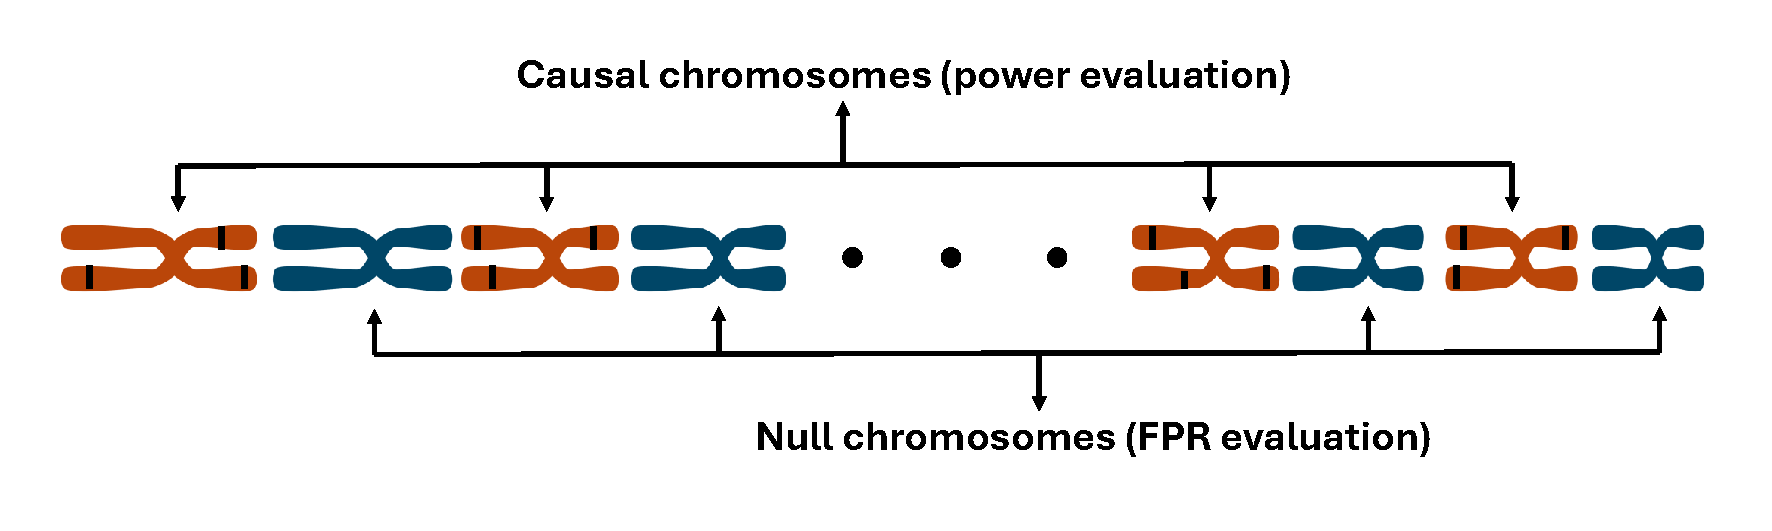
\includegraphics[width=\linewidth]{figures/thesis_qd_sim_design.pdf}
    \caption{\textbf{Phenotype simulation design.} We simulate causal effects using a spike-and-slab, mixture of Gaussian, Laplace or Gaussian distribution only on odd chromosomes, whereas we treat even chromosomes as null controls to test for false positive rate and calibration of test statistics.}
    \label{fig:qd_sim_design}
\end{figure}

In our simulations, we set the variance explained due to population stratification to be $5\%$ of trait variance, whereas sample relatedness explained 10\% of the trait variance in $2^{nd}$ degree relatives and 20\% in $1^{st}$ degree relatives \cite{jiang2019resource}.
%
To simulate a realistic MAF-dependent trait architecture, we set $c_f \propto (2f(1-f))^{\alpha}$, where $f$ is the minor allele frequency and $\alpha = -0.3$ \cite{zeng2018signatures,schoech2019quantification}.
%
For binary traits, we adopted a liability threshold model by synthesizing a quantitative phenotype as in Equation \ref{eq:sim_gen} and setting individuals above/below a given prevalence value as cases/controls.
%
We varied the prevalence in binary traits from 0.3 to 0.001 and the amount of relatedness and population structure based on the following four simulation conditions:
\begin{itemize}
    \item \textbf{Unrelated white British (GB-unrel):}
    %
    We randomly sampled $50{,}000$ individuals from the set of unrelated white British as defined in \cite{bycroft2018uk}.
    %
    This scenario does not include population structure or relatedness.
    %
    \item \textbf{Related white British (GB-rel):}
    %
    We included $25,000$ individuals from the set of individuals in the related white British but not in the unrelated white British subset, along with $25,000$ unrelated white British individuals.
    %
    This resulted in $552$ first degree, $906$ second degree, and $1396$ third degree relative pairs ($3.4 \times$ more relative pairs than randomly sampling from related white British subset). 
    %
    We also considered less and more extreme levels of relatedness, assembling sets of samples by randomly sampling from the related white British subset (referred to as GB-rel-ukb) and including high proportions of first and second degree relatives (referred as GB-rel+ having $7.3 \times$ and $4.8 \times$ more first and second degree pairs than randomly sampling from related white British subset).
    %
    \item \textbf{European structure (EUR):}
    %
    To simulate higher levels of population structure in the dataset, we included $25{,}000$ non-British European samples \cite{bycroft2018uk} along with $25{,}000$ unrelated British samples. This set also comprised $451$ first-degree and $107$ second-degree relative pairs, corresponding to $1.2 \times$ and $0.8 \times$ the amount of first- and second-degree pairs found in the subset of related white British individuals.
    %
    \item \textbf{Pan-ancestry structure (PAS):}
    %
    To simulate population structure comprising multiple ancestry descriptors found in the UK Biobank, we included $7{,}500$ self-reported African samples, $7{,}500$ self-reported South Asian samples, along with $35{,}000$ unrelated British samples, as defined in \cite{bycroft2018uk}.
    %
    This set comprised $425$ first-degree and $173$ second-degree relative pairs, corresponding to $1.1 \times$ and $1.2 \times$ more first- and second-degree pairs than randomly sampling from the subset of related white British individuals.
    %
    We simulated correlated variant effects across ancestry groups using a multivariate Gaussian, setting the covariance of effects between Africans and other subgroups to $0.4$, and between the European and south-Asian subgroups to $0.7$ \cite{ruan2022improving}.
    %
\end{itemize}
\subsection{False positive rate evaluation}
We verified the calibration of Quickdraws and the other methods by considering varying levels of polygenicity, relatedness, population structure, and the prevalence of binary traits.
%
We measured false positive rates (FPRs), calculated as the proportion of null variants (that is, variants on even chromosomes) below a chosen p-value threshold. 
%

%
We first tested calibration in analyses involving quantitative traits, considering several simulation settings with population structure and relatedness and varying polygenicity of traits from $1\%$ to $10\%$.
%
In these experiments, linear regression was not robust to the presence of relatedness and population structure, as previously observed \cite{yang2014advantages,loh2015efficient,jiang2019resource}, while all other methods were reasonably calibrated, with a few exceptions (see Figure \ref{fig:qd_sim_fpr_qt}).
%
Like other mixed-model methods, Quickdraws remained calibrated, not showing significant inflation in any of the simulation conditions we considered.
%
REGENIE produced significantly inflated test statistics in data sets including high levels of relatedness (t-test $p < 1.5 \times 10^{-4}$, see GB-rel+ in Figure \ref{fig:qd_sim_fpr_qt}), which comprise $1{,}250$ first-degree and $1{,}250$ second-degree relative pairs (corresponding to ${\sim}7.3 \times$ and ${\sim}4.8 \times$ more relatives compared to the white British subset of UK Biobank samples).
%
Finally, we observed higher variance for Quickdraws' FPR estimates in simulations involving non-homogeneous ancestry, due to higher noise in the estimated effective sample size, which relies on a smaller number of unrelated homogeneous individuals.

\begin{figure}[h!]
    \centering
    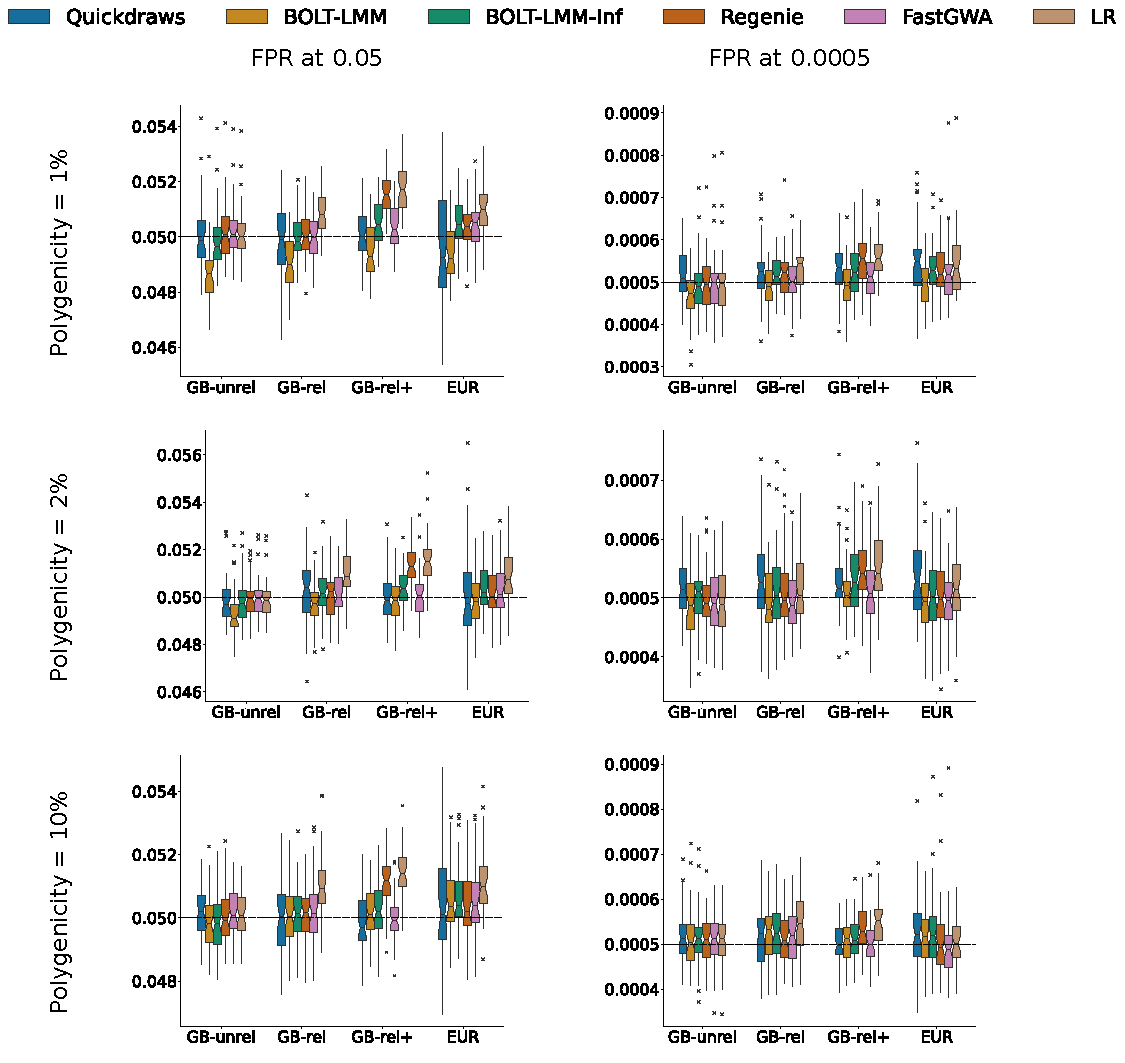
\includegraphics[width=\textwidth]{figures/sim_calibration/qt_fpr.pdf}
    
    \caption{\textbf{Summary of calibration in simulations for quantitative traits.}
    %
    False positive rate (FPR) at a significance threshold of $\alpha \in \{0.05, 0.0005\}$, calculated as the number of variants on even chromosomes with p-value lower than $\alpha$.
    %
    The line inside each box indicates the median value, the central box indicates the interquartile range, whiskers indicate data up to $1.5$ times the IQR, and outliers are shown as separate points.
    %
    A description of the group labels (GB-unrel, GB-rel, GB-rel+, EUR) is provided in Section \ref{sec:ch5-sim-design}.
    \label{fig:qd_sim_fpr_qt}
    }
\end{figure}

%
We then assessed statistical robustness in the analysis of binary traits, where we varied the prevalence of the trait from $0.3$ to $0.001$ under varying levels of population structure and relatedness (see figures \ref{fig:qd_sim_fpr_bt1} and \ref{fig:qd_sim_fpr_bt2} for FPR of common and rare variants separately) while fixing the polygenicity of the traits to 2\%. 
%
Binary trait association analysis often violates the normality assumptions made when defining the null distribution of association statistics in linear mixed models, thereby resulting in high FPR, particularly for lower frequency variants or for traits with lower prevalence \cite{zhou2018efficiently}.
%
Consistent with this, BOLT-LMM and BOLT-LMM-Inf, which are not designed for the analysis of low-prevalence binary traits, were inflated across all simulated conditions (t-test $p < 3 \times 10^{-5}$) when the prevalence dropped to or below $0.1$. 
%
Quickdraws produced controlled false positive rates for both common (MAF $> 1\%$) and rare (MAF $< 1\%$) variants in all the simulation settings we considered, which included population structure, relatedness, and low-prevalence binary traits (see figures \ref{fig:qd_sim_fpr_bt1} and \ref{fig:qd_sim_fpr_bt2} respectively).
%
REGENIE with Firth logistic regression fallback was inflated for common variants in traits with high prevalence (prevalence $=0.1$ and $0.3$) for several population structure and relatedness settings we considered.
%
When the prevalence of the trait was set to $0.01$ (that is, $500$ cases out of $50{,}000$ samples) or below, both Quickdraws and REGENIE yielded deflated test statistics (t-test $p < 3 \times 10^{-5}$); in scenarios with such a low prevalence, however, all methods we considered lacked sufficient statistical power to detect association ($\chi^2$ at causal variants ${\approx}1$).
%
SAIGE did not converge for up to $28\%$ of the traits when the prevalence dropped to $0.001$, leading to significant deflation (t-test $p < 10^{-15}$). 
%

\begin{figure}[h!]
    \centering
    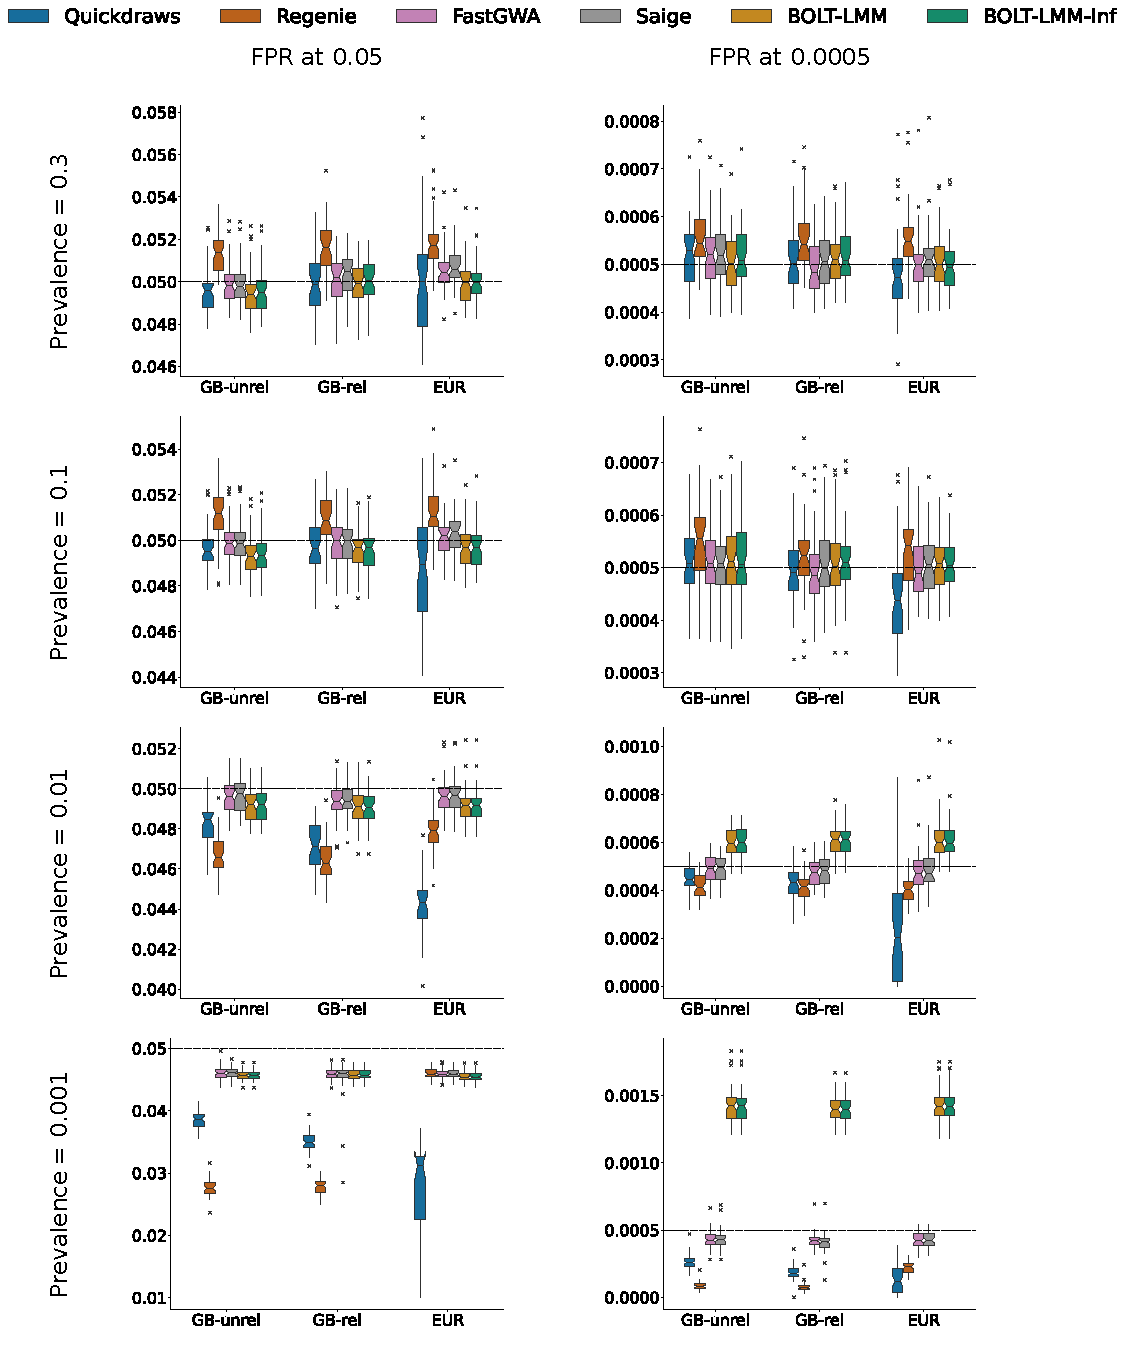
\includegraphics[width=\textwidth]{figures/sim_calibration/bt_fpr_common.pdf}
    \caption{\textbf{Summary of calibration in simulations for binary traits and common variants (MAF $\geq 1\%$).}
    %
    False positive rate (FPR) at a significance threshold of $\alpha \in \{0.05, 0.0005\}$, calculated as the number of variants on even chromosomes with p-value lower than $\alpha$.
    %
    The line inside each box indicates the median value, the central box indicates the interquartile range, whiskers indicate data up to $1.5$ times the IQR, and outliers are shown as separate points.
    %
    A description of the group labels (GB-unrel, GB-rel, EUR) is provided in Section \ref{sec:ch5-sim-design}.
    \label{fig:qd_sim_fpr_bt1}
    }
\end{figure}

\begin{figure}[h!]
    \centering
    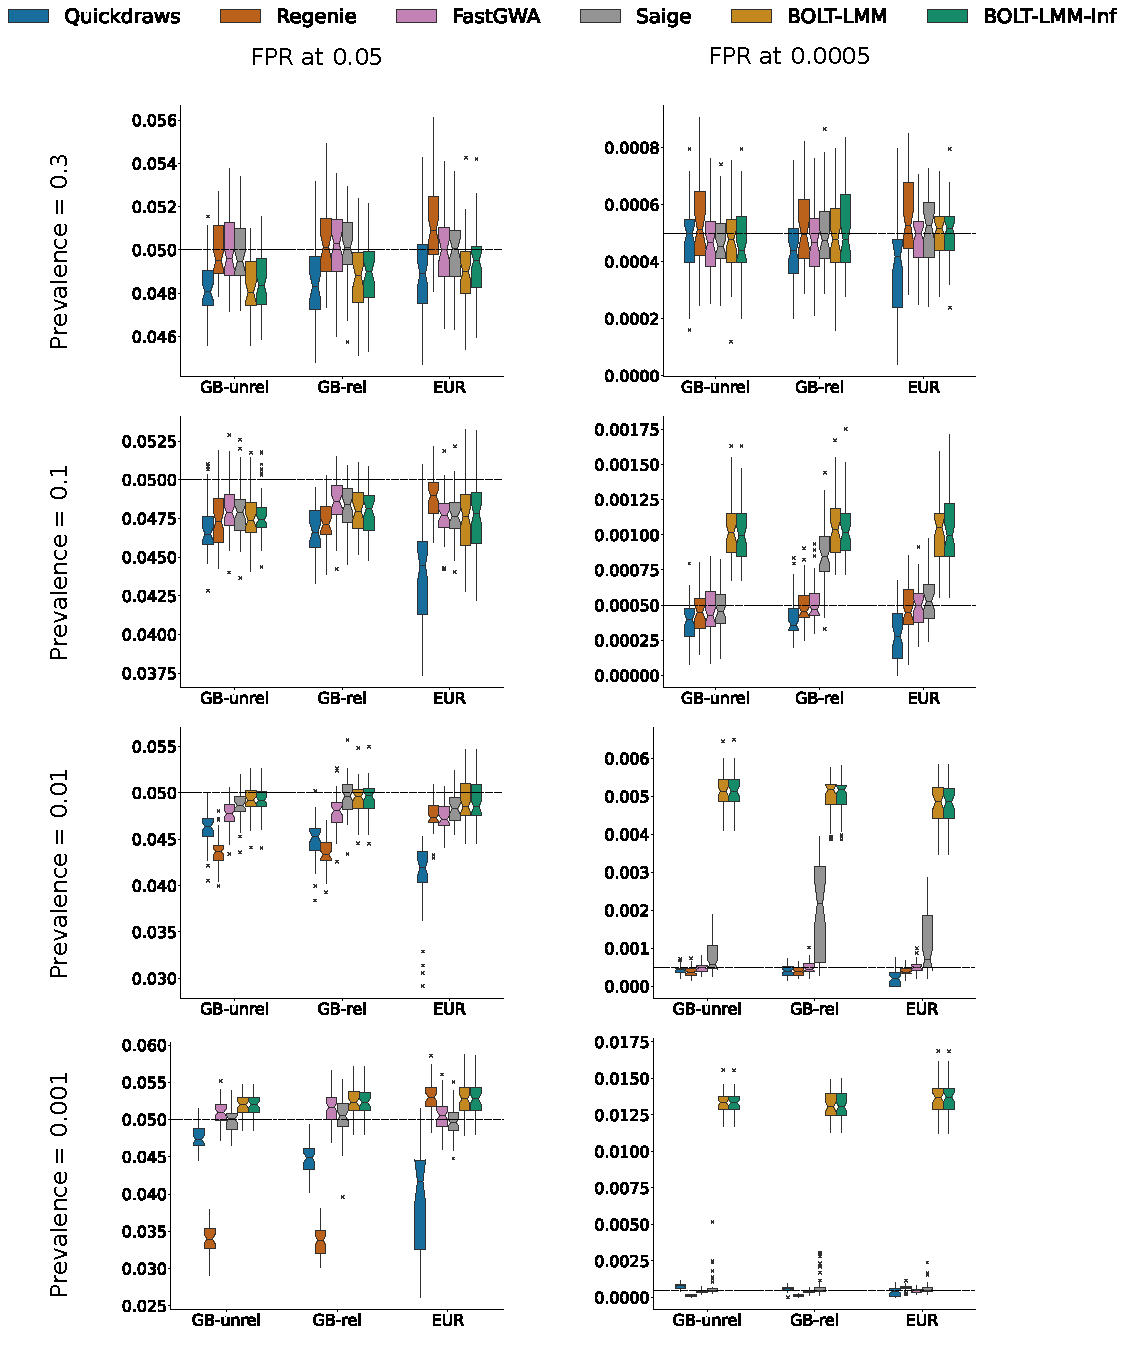
\includegraphics[width=\textwidth]{figures/sim_calibration/bt_fpr_rare.pdf}
    \caption{\textbf{Summary of calibration in simulations for binary traits and rare variants (MAF $< 1\%$).}
    %
    False positive rate (FPR) at a significance threshold of $\alpha \in \{0.05, 0.0005\}$, calculated as the number of variants on even chromosomes with p-value lower than $\alpha$.
    %
    The line inside each box indicates the median value, the central box indicates the interquartile range, whiskers indicate data up to $1.5$ times the IQR, and outliers are shown as separate points.
    %
    A description of the group labels (GB-unrel, GB-rel, EUR) is provided in Section \ref{sec:ch5-sim-design}.
    \label{fig:qd_sim_fpr_bt2}
    }
\end{figure}

%
Finally, we verified the calibration of false positive rates in various other simulated conditions, including stronger population structure with up to $30\%$ non-European ancestry (see Figure \ref{fig:sim_calib_pop}), varying levels of relatedness (see Figure \ref{fig:sim_calib_rel}), and genetic architectures involving diverse causal effect size distributions (see Figure \ref{fig:sim_calib_mog}).
%
We also evaluated false positive rates in simulations involving all white British individuals (N $\approx 405k$) and all self-identified European individuals from the UK Biobank (N $\approx 460k$), varying levels of polygenicity in quantitative traits ($1\%$ to $10\%$), and varying levels of prevalence ($0.3$ to $0.001$) in binary traits. We found Quickdraws to yield controlled false positive rates across varying significance thresholds, while fastGWA, REGENIE, and BOLT-LMM-Inf led to significant inflation in some cases (see figures \ref{fig:sim_400k}, \ref{fig:sim_460k} and tables \ref{tab:fpr_simulations}, \ref{tab:fgwa_fpr_sims}).
%
This is likely the result of residual population stratification, which is not fully corrected using principal components in these simulated scenarios and, if present, may cause subtle inflation in real-data analyses \cite{haworth2019apparent,sohail2019polygenic,berg2019reduced}.

\begingroup
\renewcommand{\arraystretch}{1.2} % Locally increases the row spacing just for this table

\begin{table}[h!]
\centering
\caption{
\textbf{Summary of calibration in simulations involving (a) $N=405$k white British individuals and (b) $N=460$k European individuals \cite{bycroft2018uk}.} We report the false positive rate (FPR) at a significance threshold of $\alpha \in \{0.05, 0.0005\}$, calculated as the fraction of variants on even chromosomes with p-value lower than $\alpha$.
%
We varied the polygenicity from $1\%$ to $10\%$ in quantitative traits.
%
For binary traits, we changed the prevalence from $0.3$ to $0.001$, fixing the polygenicity to 2\%.
%
Mean FPR refers to the mean across $50$ independent simulated traits, SE refers to standard errors, and p-values are computed for the significance of a deviation from the FPR threshold.
}
\begin{subtable}[h]{\textwidth}
            \centering
\resizebox{\textwidth}{!}{
\begin{tabular}{|c|c|c|c|c|c|}
\hline
\textbf{Simulation Type} & \textbf{FPR Threshold} & \textbf{Polygenicity (QT) / } & \textbf{Mean} & \textbf{SE} & \textbf{T-test} \\ 
 &  & \textbf{Prevalence (BT)} & \textbf{FPR} & \textbf{FPR}  & \textbf{P} \\ 
\hline
\multirow{6}{*}{Quantitative Traits} & \multirow{3}{*}{0.05}  & 1\%   & 0.05034 & 0.00022 & 0.13382 \\ \cline{3-6}
                                     &                        & 2\%   & 0.05040 & 0.00029 & 0.17865 \\ \cline{3-6}
                                     &                        & 10\%  & 0.05036 & 0.00017 & 0.03658 \\ \cline{2-6}
                                     & \multirow{3}{*}{0.0005}& 1\%   & 0.00052 & 0.00001 & 0.06363 \\ \cline{3-6}
                                     &                        & 2\%   & 0.00053 & 0.00002 & 0.04845 \\ \cline{3-6}
                                     &                        & 10\%  & 0.00052 & 0.00001 & 0.04787 \\ \hline
\multirow{8}{*}{Binary Traits}       & \multirow{4}{*}{0.05}  & 0.3   & 0.04923 & 0.00022 & 0.00103 \\ \cline{3-6}
                                     &                        & 0.1   & 0.04986 & 0.00019 & 0.46758 \\ \cline{3-6}
                                     &                        & 0.01  & 0.04940 & 0.00016 & 0.00044 \\ \cline{3-6}
                                     &                        & 0.001 & 0.04648 & 0.00016 & $7.39 \times 10^{-39}$ \\ \cline{2-6}
                                     & \multirow{4}{*}{0.0005}& 0.3   & 0.00048 & 0.00001 & 0.05193 \\ \cline{3-6}
                                     &                        & 0.1   & 0.00051 & 0.00001 & 0.57445 \\ \cline{3-6}
                                     &                        & 0.01  & 0.00046 & 0.00001 & 0.00018 \\ \cline{3-6}
                                     &                        & 0.001 & 0.00042 & 0.00001 & $5.28 \times 10^{-13}$ \\ \hline
\end{tabular}
}
\caption{$N=405$k white British individuals.}
\end{subtable}

\vspace{7mm}

\begin{subtable}[h]{\textwidth}
            \centering
\resizebox{\textwidth}{!}{
\begin{tabular}{|c|c|c|c|c|c|}
\hline
\textbf{Simulation Type} & \textbf{FPR Threshold} & \textbf{Polygenicity (QT) / } & \textbf{Mean} & \textbf{SE} & \textbf{T-test} \\ 
 &  & \textbf{Prevalence (BT)} & \textbf{FPR} & \textbf{FPR}  & \textbf{P} \\ 
\hline
\multirow{6}{*}{Quantitative Traits} & \multirow{3}{*}{0.05}  & 1\%   & 0.05061 & 0.000231 & 0.0098 \\ \cline{3-6}
                                     &                        & 2\%   &0.05019 & 0.00025 & 0.4444 \\ \cline{3-6}
                                     &                        & 10\%  &  0.05037 & 0.00026 & 0.1709 \\ \cline{2-6}
                                     & \multirow{3}{*}{0.0005}& 1\%   & 0.00053 & 0.00001 &  0.0075 \\ \cline{3-6}
                                     &                        & 2\%   & 0.00053 & 0.00001 & 0.01728 \\ \cline{3-6}
                                     &                        & 10\%  &  0.00053 & 0.00001 &  0.0429 \\ \hline
\multirow{8}{*}{Binary Traits}       & \multirow{4}{*}{0.05}  & 0.3   & 0.04983 & 0.00015 & 0.3108 \\ \cline{3-6}
                                     &                        & 0.1   & 0.04997 & 0.00017 & 0.9015 \\ \cline{3-6}
                                     &                        & 0.01  & 0.0437 & 0.00058 & $5.19 \times 10^{-18}$ \\ \cline{3-6}
                                     &                        & 0.001 & 0.03121 & 0.0022 & $3.72 \times 10^{-13} $ \\ \cline{2-6}
                                     & \multirow{4}{*}{0.0005}& 0.3   & 0.00051 & 0.00001 & 0.1391 \\ \cline{3-6}
                                     &                        & 0.1   & 0.00053 & 0.00002 & 0.0436 \\ \cline{3-6}
                                     &                        & 0.01  & 0.00033 & 0.00003 & $4.93 \times 10^{-7}$ \\ \cline{3-6}
                                     &                        & 0.001 & 0.00022 & 0.00003 & $2.47 \times 10^{-15}$ \\ \hline
\end{tabular}
}
\caption{$N=460$k European individuals.}
\end{subtable}

\label{tab:fpr_simulations}
\end{table}

\endgroup % Ends the local redefinition of \arraystretch

\clearpage

\subsection{Statistical power evaluation}
We now focus on evaluating the statistical power of Quickdraws in these simulations.
%
We first tested the performance of Quickdraws in quantitative trait association and compared it with previous association testing methods including BOLT-LMM, REGENIE, FastGWA, and an implementation of linear regression provided in Plink \cite{purcell2007plink,chang2015second}.
%
For BOLT-LMM, we also considered a faster implementation that uses infinitesimal priors (BOLT-LMM-Inf), which is more scalable but does not lead to higher association power in less polygenic genetic architectures \cite{loh2015efficient,loh2018mixed}.
%
We measured statistical power by considering the average $\chi^2$ test statistics at simulated causal variants, focusing on the set of unrelated white British samples and varying the number of causal variants in the simulation from $5{,}000$ to $50{,}000$ \cite{zeng2018signatures}.
%
We normalized the average $\chi^2$ test statistics at causal variants by the average $\chi^2$ test statistics at null variants to remove any residual stratification.
%
In these simulations, the modeling of trait polygenicity adopted by Quickdraws led to higher average $\chi^2$ statistics (paired t-test $p < 10^ {-20}$ for polygenicity up to $2\%$) compared to REGENIE, FastGWA, BOLT-LMM-Inf, and linear regression (see Figure \ref{fig:sim2_1} and Figure \ref{fig:sim_power_qt} for more simulation conditions).
%
The difference in association power compared to other infinitesimal methods was larger for traits with lower polygenicity (paired t-test $p < 10^{-53}$ for $5{,}000$ causal variants).
%
For instance, when the number of causal variants was reduced to ${5{,}000}$, Quickdraws achieved $\geq 11.46\%$ higher average $\chi^2$ compared to REGENIE and BOLT-LMM-Inf (paired t-test $p < 10^{-53}$), resulting in a similarly large gain in effective sample size \cite{yang2011genomic}.
%

%
Next, we applied Quickdraws to the analysis of binary traits, comparing its association power with previous binary trait association methods including SAIGE, REGENIE, and FastGWA-GLMM.
%
We simulated phenotypes under a liability threshold model, where cases and controls are defined as individuals who are above or below a chosen liability threshold as described in Section \ref{sec:ch5-sim-design}.
%
We fixed the prevalence at $0.3$ and varied the number of causal variants in the simulation from $1{,}250$ to $10{,}000$ \cite{stahl2012bayesian, zeng2018signatures, o2019extreme}.
%
In these experiments, the use of a non-infinitesimal prior in Quickdraws led to higher statistical power compared to SAIGE, REGENIE, and FastGWA (paired t-test $p < 10^{-12}$, Figure \ref{fig:sim2_2} and Figure \ref{fig:sim_power_bt} for more simulation conditions).
%
The difference in association power compared to other methods was again larger for traits with lower polygenicity (paired t-test $p < 10^{-43}$ for $1{,}250$ and $2{,}500$ causal variants).
%
For instance, Quickdraws obtained $11.5\%$ and $12.04\%$ higher average $\chi^2$ compared to REGENIE and FastGWA on the simulated causal variants for traits with a low polygenicity of $0.25\%$.

\begin{figure}[h!]
    \centering
    % 
\includegraphics[scale=0.335]{figures/sim_power/legend.png}
    \begin{subfigure}{.5\textwidth}
    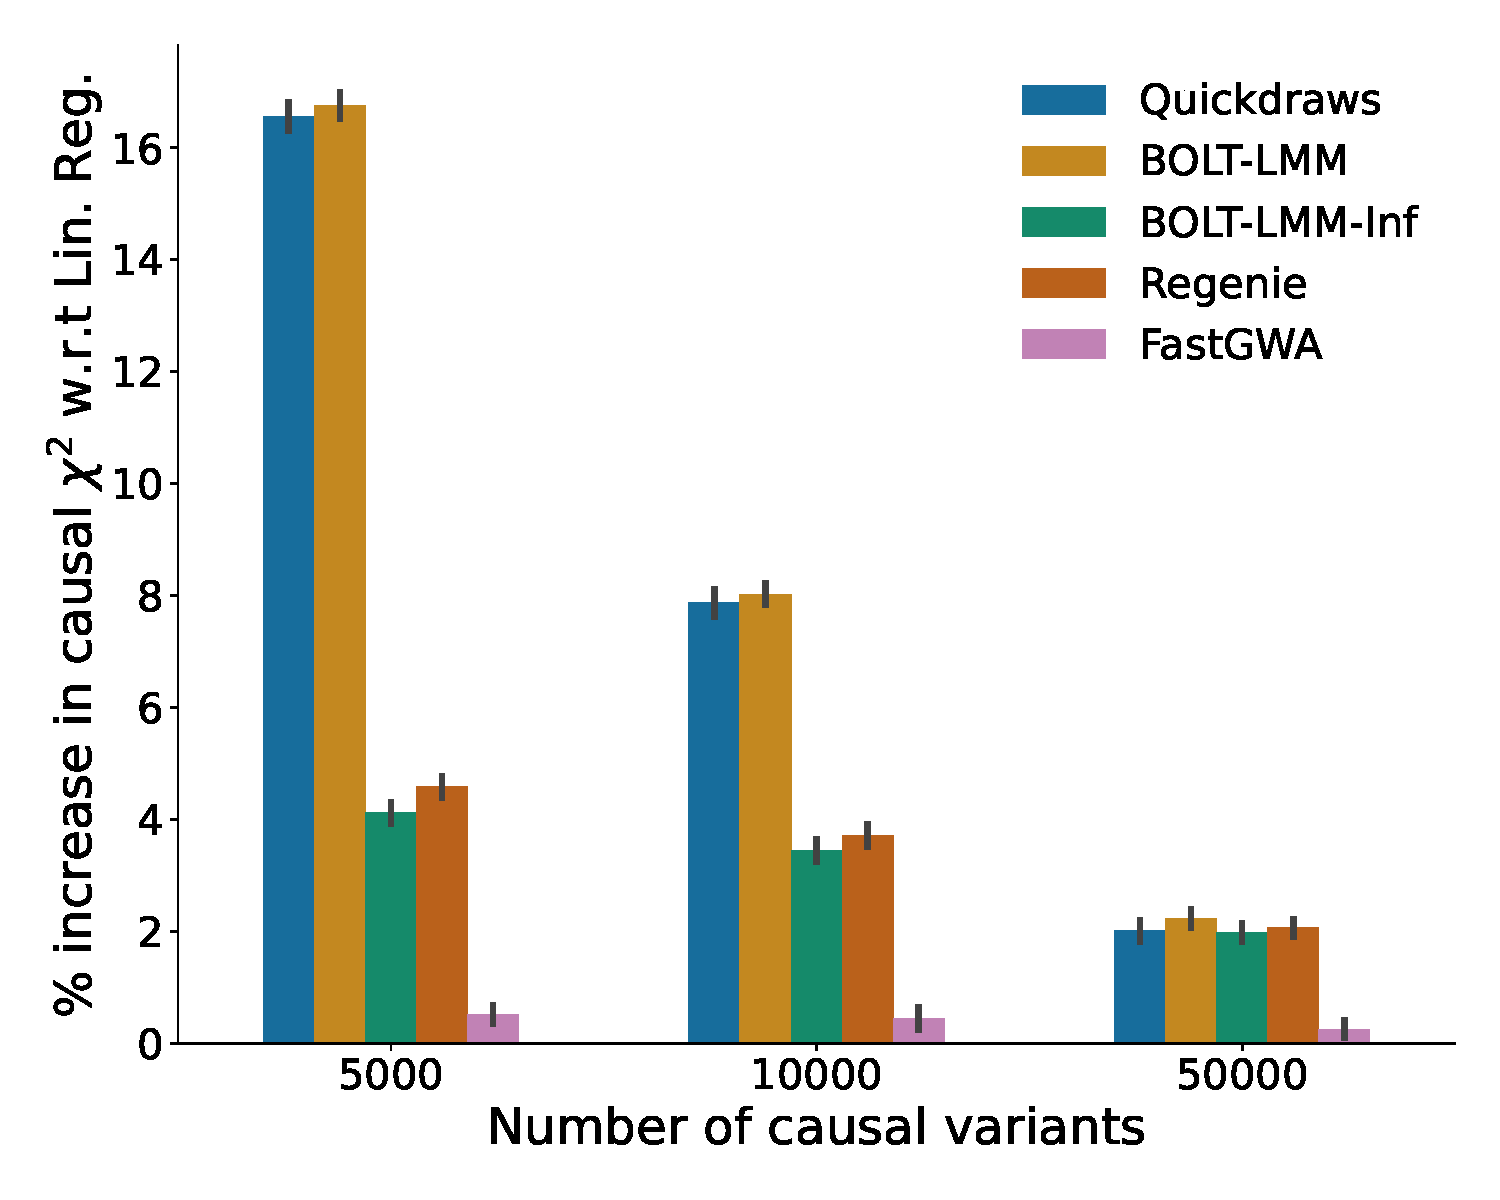
\includegraphics[scale=0.29]{figures/sim_power/paper_result_power_50000.pdf}
    \caption{}
    \label{fig:sim2_1}
    \end{subfigure}%
    \begin{subfigure}{.5\textwidth}
    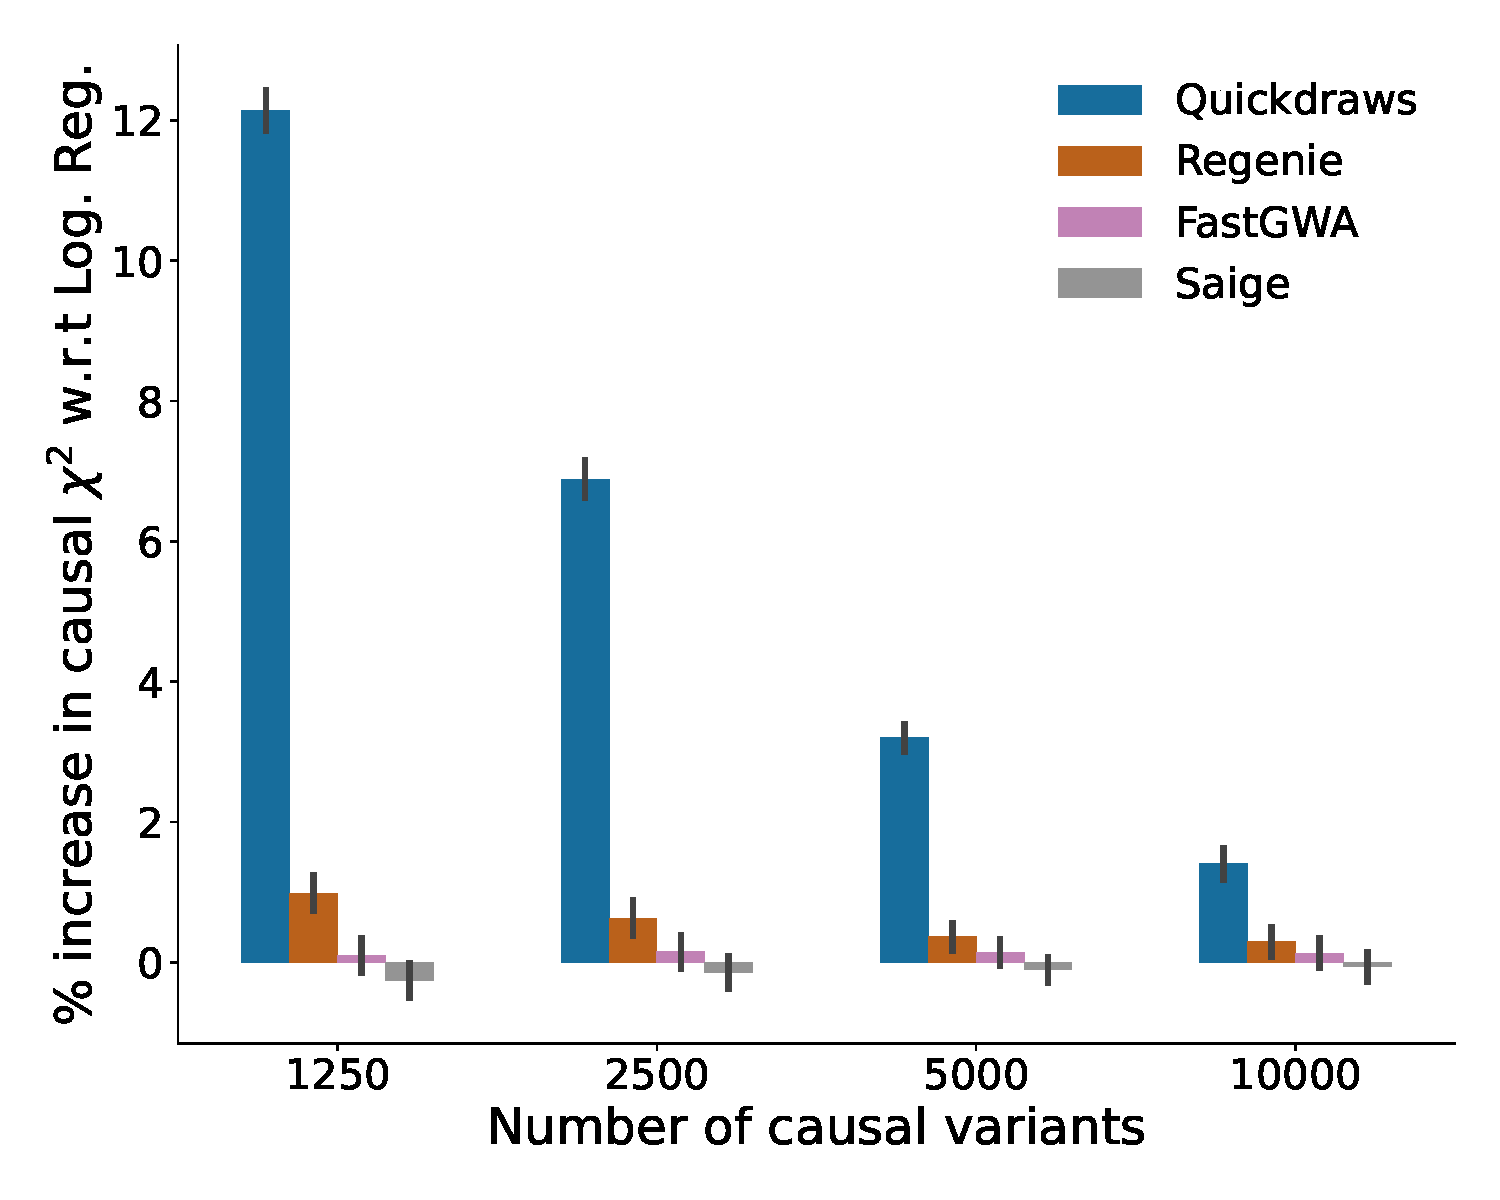
\includegraphics[scale=0.29]{figures/sim_power/paper_result_power_10000.pdf}
    \caption{}
    \label{fig:sim2_2}
    \end{subfigure}
    % \includegraphics[width=\textwidth]{figures/loya_qd_fig1.pdf}
    \caption{\textbf{Statistical power in simulated quantitative and binary traits for unrelated British samples.}
    %
    (a) \% increase in average $\chi^2$ test statistics at causal variants with respect to\ linear regression (Lin. Reg.) for quantitative traits, varying the number of simulated causal variants from $5{,}000$ to $50{,}000$ variants.
    %
    (b) \% increase in average $\chi^2$ test-statistics at causal variants with respect to\ logistic regression (Log. Reg.) for binary traits, varying the number of simulated causal variants from $1{,}250$ to $10{,}000$ variants.
    %
    Traits in panel (a) and (b) are simulated for $50{,}000$ samples with $h^2 = 0.4$; the prevalence is fixed to $30$\% for binary traits in panel (b).
    %
    Error bars represent the standard error in the percentage improvement, measured using $50$ independent traits.
    %
    The causal $\chi^2$ is normalized by the mean $\chi^2$ at null variants for each trait.
    %
    } 
    \label{fig:sim_power}
\end{figure}

%
Finally, we tested Quickdraws in simulations where causal effects were not assumed to follow a spike-and-slab distribution, where a subset of variants contributes to the phenotype.
%
Instead, we sampled effects from a Gaussian, a mixture of Gaussian, or a Laplace distribution.
%
In the mixture of Gaussian setting, we again observed that Quickdraws and BOLT-LMM yielded higher power compared to other models.
%
In simulations involving fully infinitesimal traits with Laplace and Gaussian effects, Quickdraws and BOLT-LMM produced results similar to other approaches that assume a fully infinitesimal trait architecture (see Figure \ref{fig:sim_power_mog}).
%
We also evaluated power in simulations involving all white British individuals from the UK Biobank ($N \approx 405$k) and all self-identified European individuals from the UK Biobank ($N \approx 460$k).
%
In these settings, we found Quickdraws to provide the highest association power, with higher power than BOLT-LMM when the polygenicity of the trait was low (see figures \ref{fig:sim_400k} and \ref{fig:sim_460k}).
%
%



Overall, these simulations demonstrate that the use of a non-infinitesimal spike-and-slab prior results in higher statistical power to detect association in both quantitative and binary trait simulations.
%
Quickdraws matched or outperformed the power of BOLT-LMM in the analysis of quantitative traits and obtained higher association power than existing GWAS algorithms in binary traits.
%
Quickdraws also yielded controlled FPR in all simulation settings we considered, which included population structure, relatedness, and low-prevalence binary traits.

\begin{figure}[h!]
    \centering
    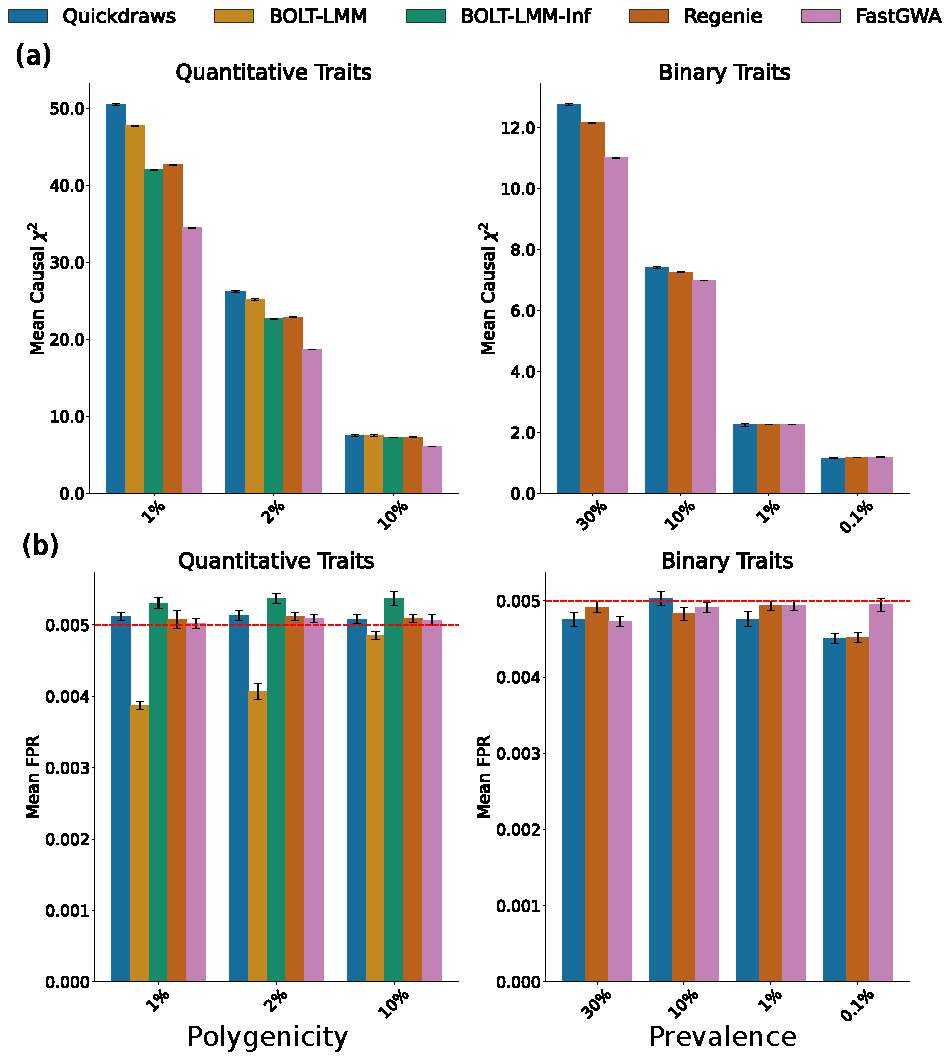
\includegraphics[width=\textwidth]{figures/qd_panel_sim.pdf}
    \caption{\textbf{Power and FPR in N$=405$k simulation.}
    %
    (a) The mean $\chi^2$ at causal variants across different methods and polygenicities for Quantitative traits, and prevalence for binary traits. The $\chi^2$ at causal variants is not normalized by the $\chi^2$ at null variants in this plot.
    %
    (b) The mean false positive rates (FPR) at 0.005 calculated at null variants across different methods and polygenicities for Quantitative traits, and prevalence for binary traits.
    %
    The simulation was performed using the N$=405$k set of white British individuals. The error bars represent 95\% confidence intervals.
    %
    The red dashed line corresponds to false positive rate $=0.005$.
    }
    \label{fig:sim_400k}
\end{figure}

\begin{figure}[h]
    \centering
    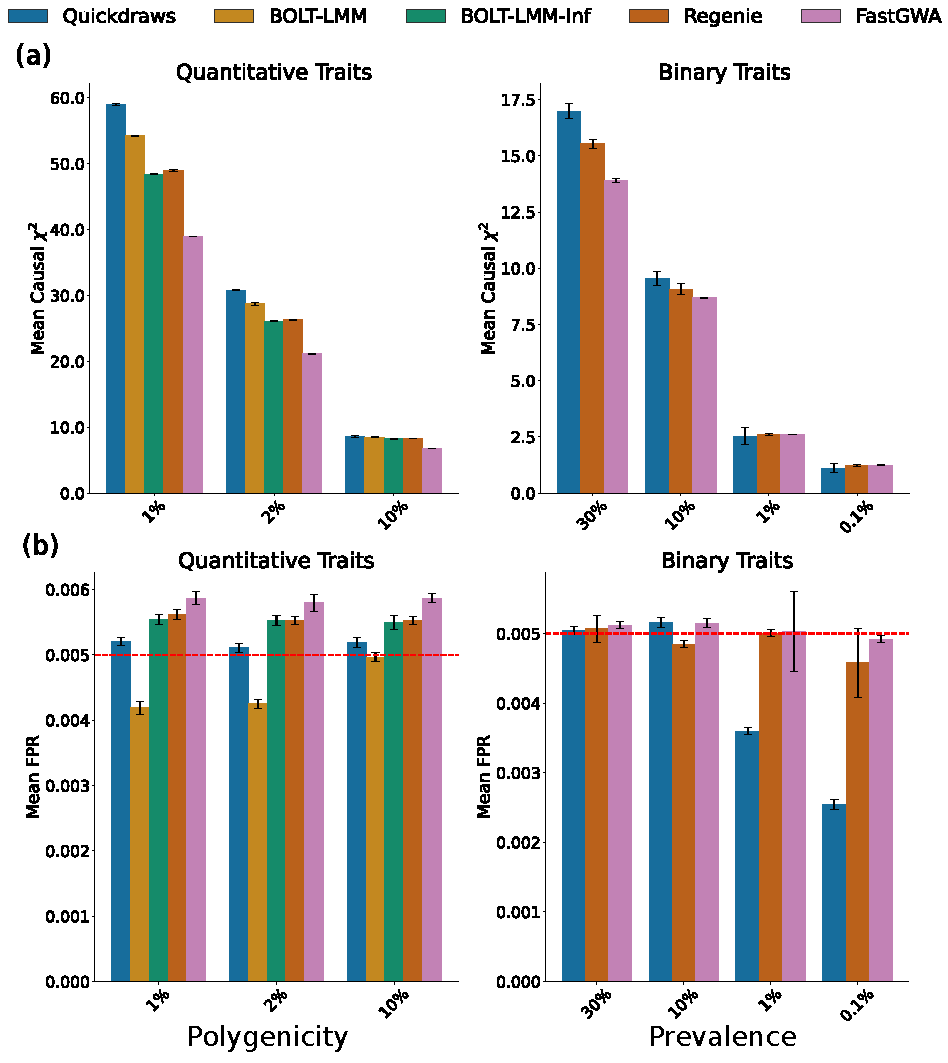
\includegraphics[scale=1]{figures/qd_panel_sim2.pdf}
    \caption{\textbf{Power and FPR in N$=460$k simulation.}
    %
    (a) The mean $\chi^2$ at causal variants across different methods and polygenicities for quantitative traits, and prevalence for binary traits. The $\chi^2$ at causal variants is not normalized by the $\chi^2$ at null variants in this plot.
    %
    (b) The mean false positive rates (FPR) at 0.005 calculated at null variants across different methods and polygenicities for Quantitative traits, and prevalence for binary traits.
    %
    The simulation was performed using the N$=460$k set of UK Biobank self-identified Europeans \cite{bycroft2018uk}. The error bars represent 95\% confidence intervals.
    %
    The red dashed line corresponds to false positive rate $=0.005$.
    }
    \label{fig:sim_460k}
\end{figure}

\clearpage

\section{UK Biobank analysis}
\label{sec:ch5-ukb}

We applied Quickdraws to the analysis of $79$ quantitative traits (comprising of blood-related, anthropometric, and other traits) and $50$ self-reported disease traits for ${\sim}405{,}000$ white British individuals from the UK Biobank dataset (see tables \ref{tab:ukb_qt_traits} and \ref{tab:ukb_bt_traits} for the list of traits), which we selected based on their high phenotyping rate and the significance of their estimated heritability as described in Section \ref{sec:ch5-data}.
%
We applied standard quality-control filtering steps, retaining $458{,}420$ genotyped markers to be used for model-fitting and ${\sim}13.3$ million imputed variants for association testing.
%
We compared the test statistics we obtained using Quickdraws to those obtained by other association methods, including SAIGE, FastGWA, REGENIE, and BOLT-LMM.
%

\subsection{Analysis of false positive rates}
%
We assessed the calibration of the test-statistics in real data by comparing the LD-score regression attenuation ratio estimates \cite{loh2018mixed} obtained using Quickdraws to those obtained using linear regression while restricting to the set of unrelated individuals with homogeneous British ancestry \cite{bycroft2018uk}.
%
Because linear regression is expected to be calibrated in this sample set, similar attenuation ratio estimates for Quickdraws provide evidence for its calibration \cite{loh2018mixed,jiang2019resource}.
%
We performed LD-score regression using the baseline-LD model \cite{gazal2017linkage} and estimated attenuation ratios using test statistics generated using Quickdraws on all ${\sim}13.3$ million testing variants across the set of $79$ quantitative traits.
%
Quickdraws produced attenuation ratios close to those of linear regression on unrelated samples (mean attenuation ratio for Quickdraws $ = 0.0832$, s.e.\ $= 0.008$; mean attenuation ratio for linear regression on unrelated samples $= 0.0892$, s.e.\ $= 0.008$; Figure \ref{fig:real1c}). 
%
Quickdraws also remained calibrated in the analysis of low-prevalence binary traits, where it did not produce signatures of false positive association signals that are present in methods that do not perform adjustments of test statistics such as saddle-point approximation (SPA) \cite{zhou2018efficiently} or approximate Firth logistic regression \cite{mbatchou2021computationally} (see Manhattan plots in figures \ref{fig:qd_man_bin1} and \ref{fig:qd_man_bin2}, additional examples of Manhattan plots for quantitative trait are shown in figures \ref{fig:qd_man_quant1} and  \ref{fig:qd_man_quant2}).
%

\begin{figure}
    \centering
    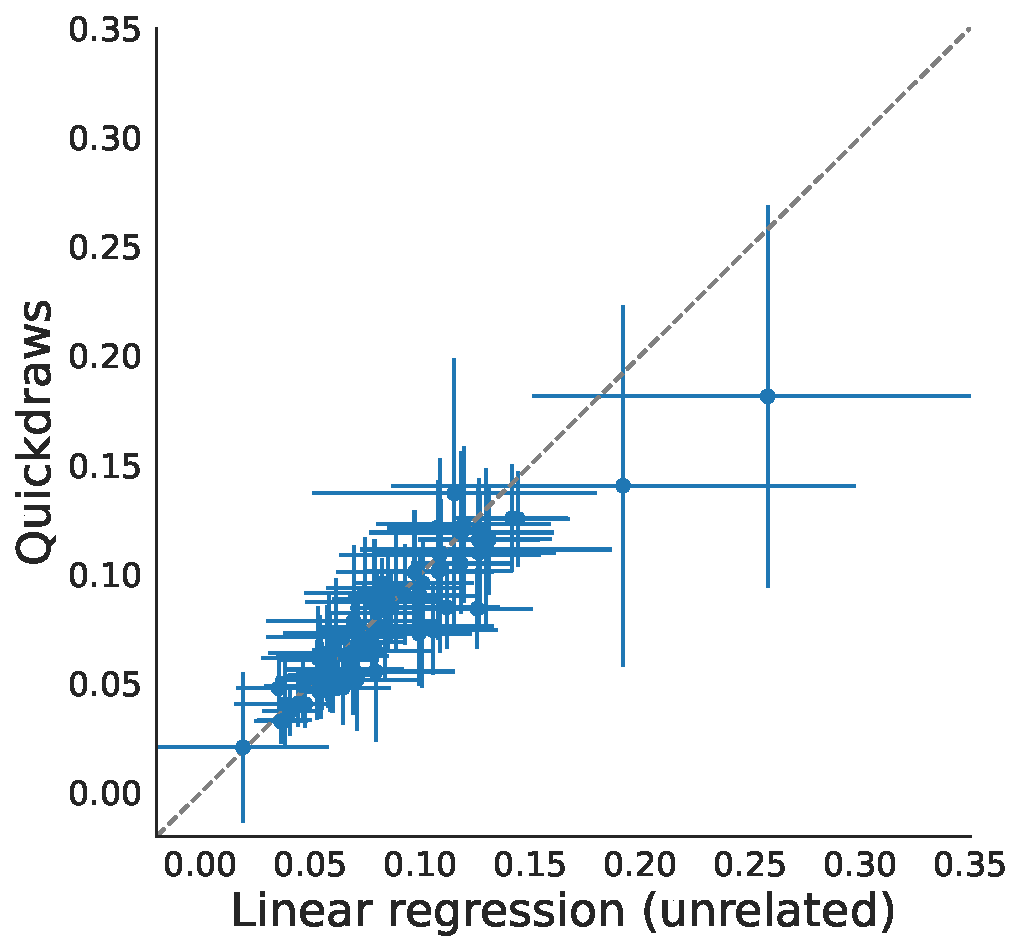
\includegraphics[width=0.65\linewidth]{figures/qd_ukb/attnratio_plot.pdf}
    \caption{\textbf{Calibration in real data analysis.} Attenuation ratio of Quickdraws (N=$405$k) vs. linear regression in unrelated samples (N=$337$k); vertical and horizontal lines represent mean $\pm$ standard errors in the attenuation ratio estimate for each method.}
    \label{fig:real1c}
\end{figure}

%
To further validate signals found using Quickdraws but not found using REGENIE, we evaluated the functional annotation of regions where these variants are found.
%
We used the Baseline-LD model annotations \cite{finucane2015partitioning,gazal2017linkage} to assess the distribution of functional annotations for sets of variants associated using different methods.
%
We define the functional enrichment for a set of variants as the proportion of variants being in a particular functional category, divided by the genome-wide fraction of variants assigned to that category.
%
We considered binary and quantitative traits separately and estimated the mean functional enrichment across phenotypes by computing the ratio between the number of variants from a given set that belong to a functional category (numerator) and the total number of variants in the set (denominator).
%
We estimated this ratio by separately summing the numerator and denominator term across all analyzed phenotypes.
%
We estimated standard errors around the enrichment by applying the jackknife method to $50$ equally sized genome blocks.
%
We looked at functional enrichment for various sets of variants, including (1) variants found in Quickdraws but not in REGENIE, (2) variants found in both Quickdraws and REGENIE.
%
For (2), we matched the $\chi^2$ distribution of the two considered sets, sampling variants detected using REGENIE so that they approximately match the empirical $\chi^2$ distribution of the variants detected using Quickdraws.
%
We found similar enrichments compared to variants found using both REGENIE and Quickdraws (see figures \ref{fig:functional_qt} and \ref{fig:functional_bt}), suggesting no substantial differences in the functional profile of variants exclusively detected using Quickdraws.
%

\begin{figure}[h!]
    \centering
    \begin{subfigure}{0.5\textwidth}
    \captionsetup{justification=raggedright,singlelinecheck=false}
    \caption*{\textbf{(a)}}
    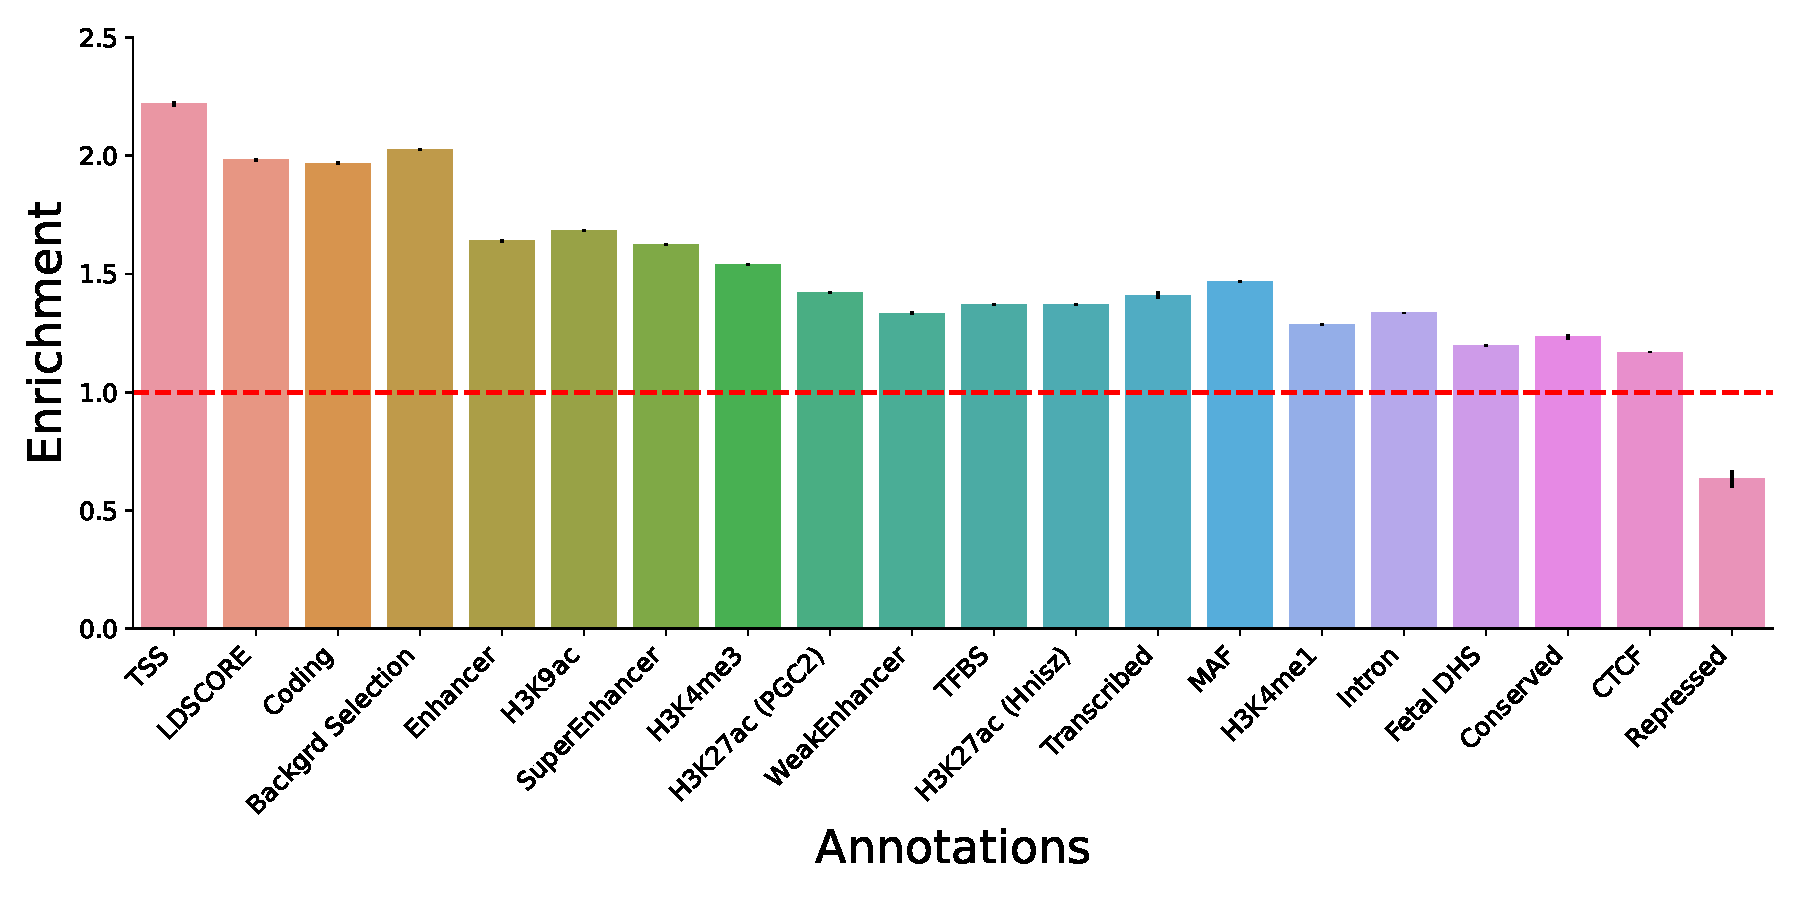
\includegraphics[width=\textwidth]{figures/functional/annotation_both_quant.pdf}
    \end{subfigure}%
    \begin{subfigure}{0.5\textwidth}
    \captionsetup{justification=raggedright,singlelinecheck=false}
    \caption*{\textbf{(b)}}
    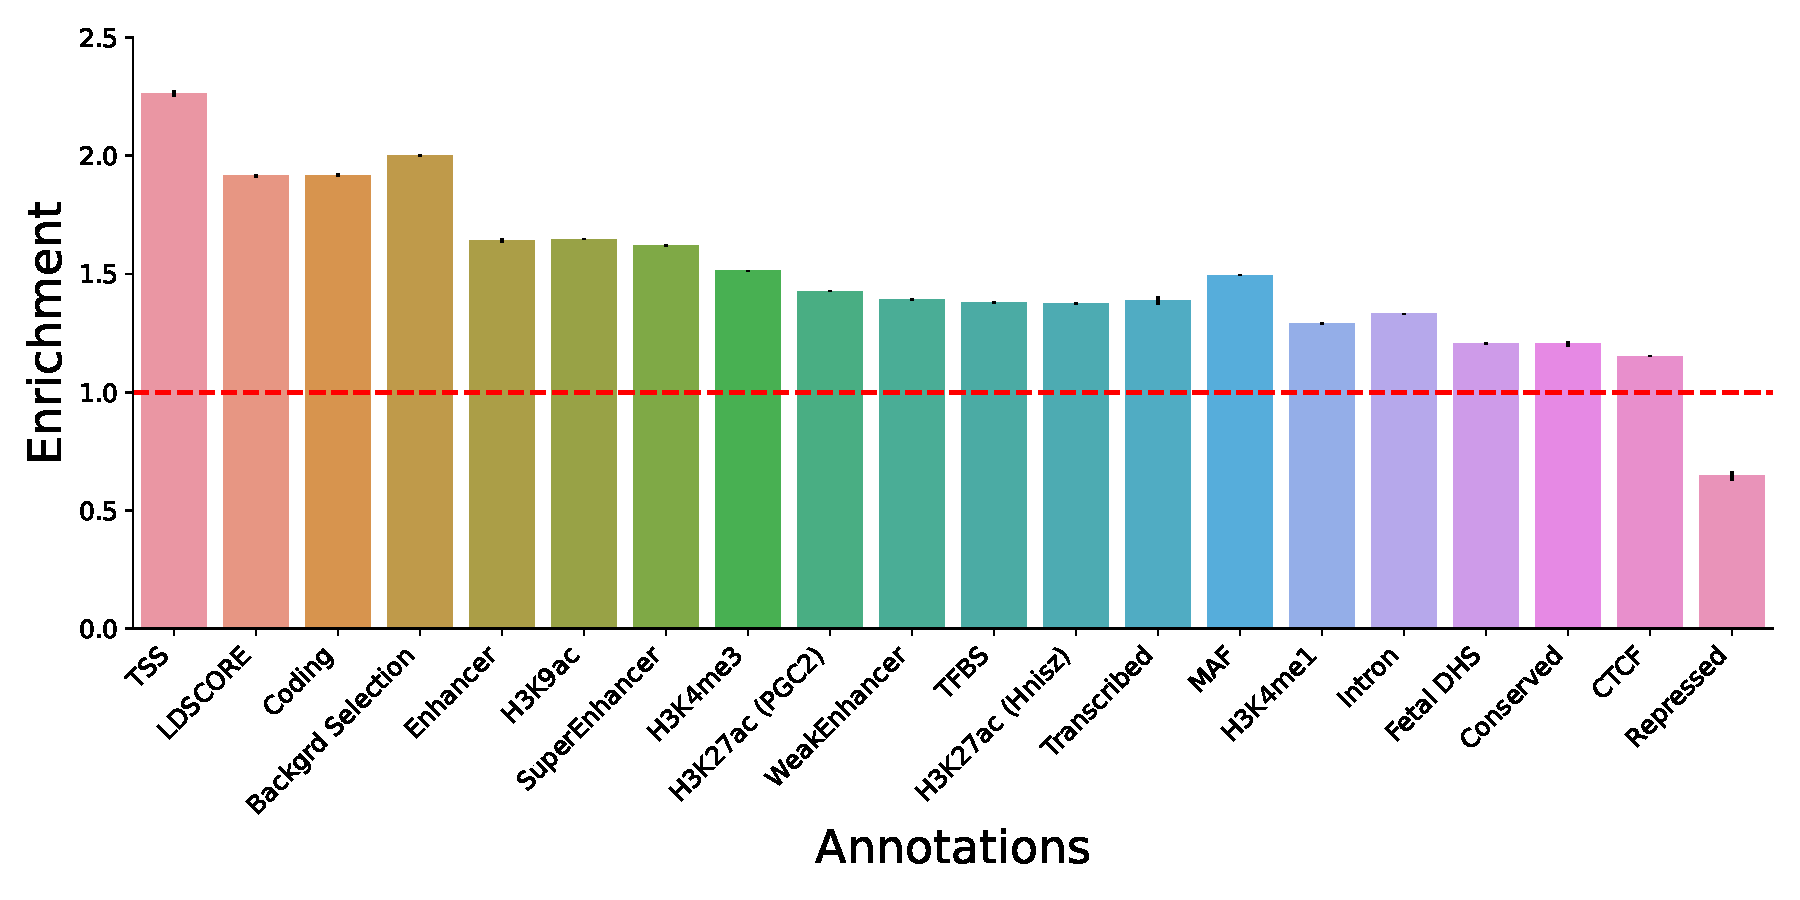
\includegraphics[width=\textwidth]{figures/functional/annotation_onlyqd_quant.pdf}
    \end{subfigure}
    \caption{\textbf{Functional enrichment at associated variants for quantitative traits.}
    %
    Functional enrichment profile of variants associated across $79$ quantitative traits.
    %
    We considered either (a) the set of variants significantly associated ($p \leq 5 \times 10^{-8}$) using both Quickdraws and REGENIE, matching the p-value distribution (see Methods), or (b) the set of variants associated using Quickdraws but not REGENIE.
    %
    Error bars represent jackknife standard errors; the red dashed line corresponds to no enrichment.
    }
    \label{fig:functional_qt}
\end{figure}

\begin{figure}[h!]
    \centering
    \begin{subfigure}{0.5\textwidth}
    \captionsetup{justification=raggedright,singlelinecheck=false}
    \caption*{\textbf{(a)}}
    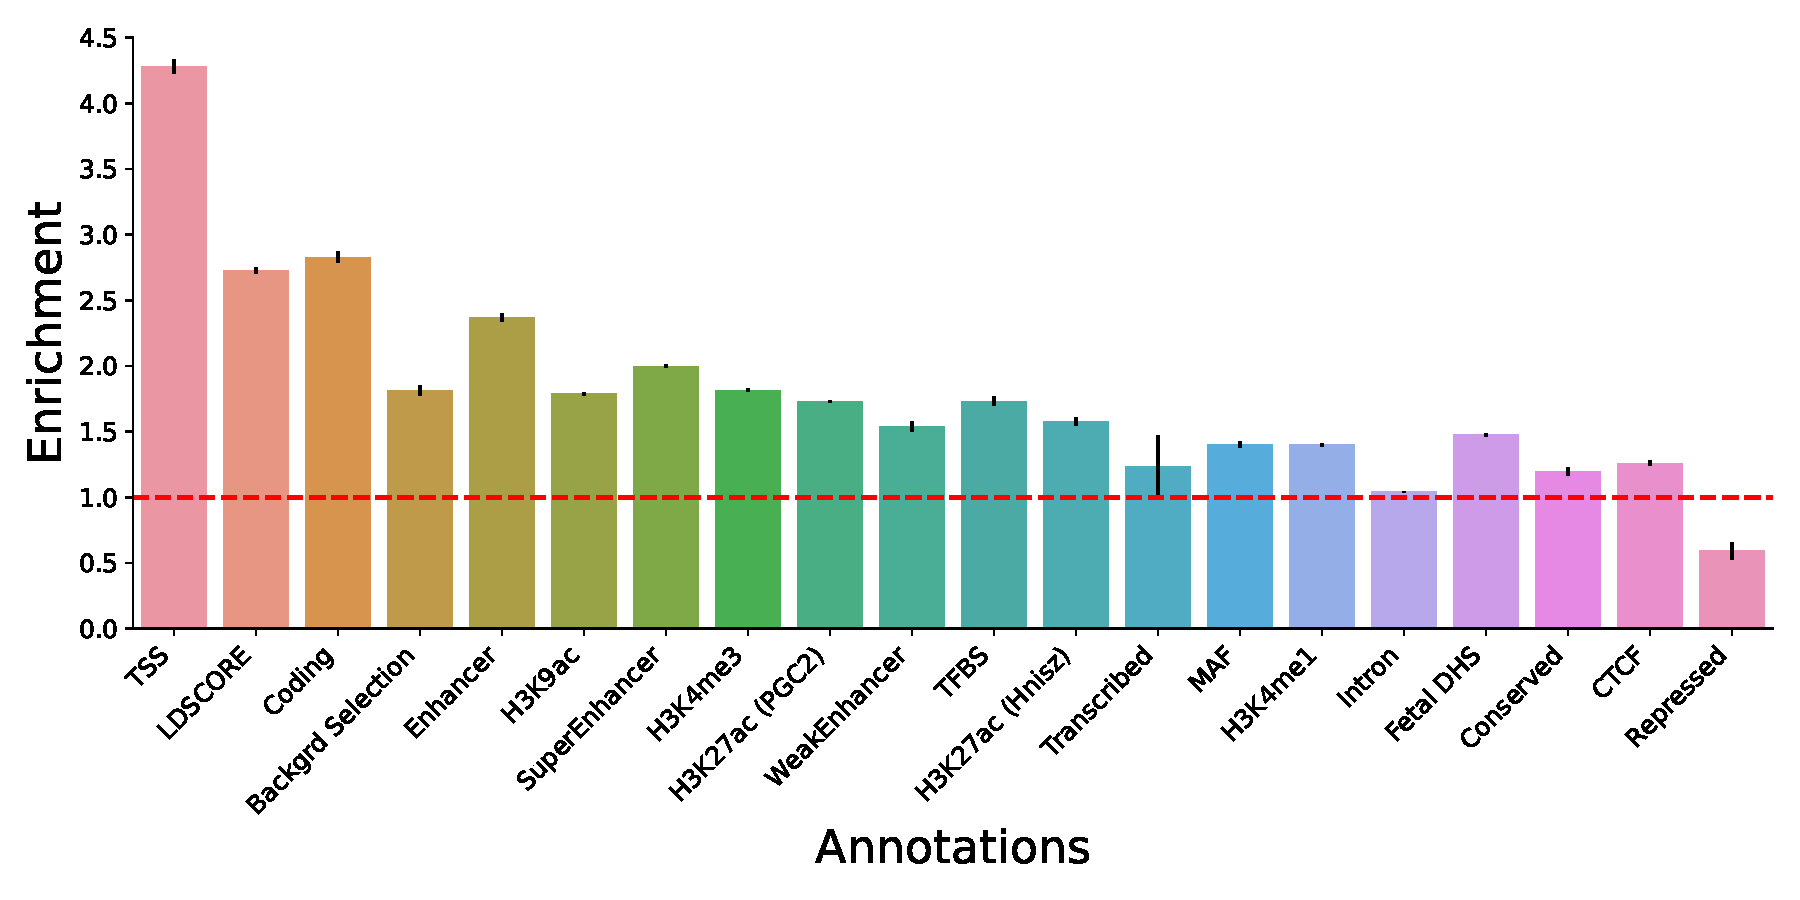
\includegraphics[width=\textwidth]{figures/functional/annotation_both_binary.pdf}
    \end{subfigure}%
    \begin{subfigure}{0.5\textwidth}
    \captionsetup{justification=raggedright,singlelinecheck=false}
    \caption*{\textbf{(b)}}
    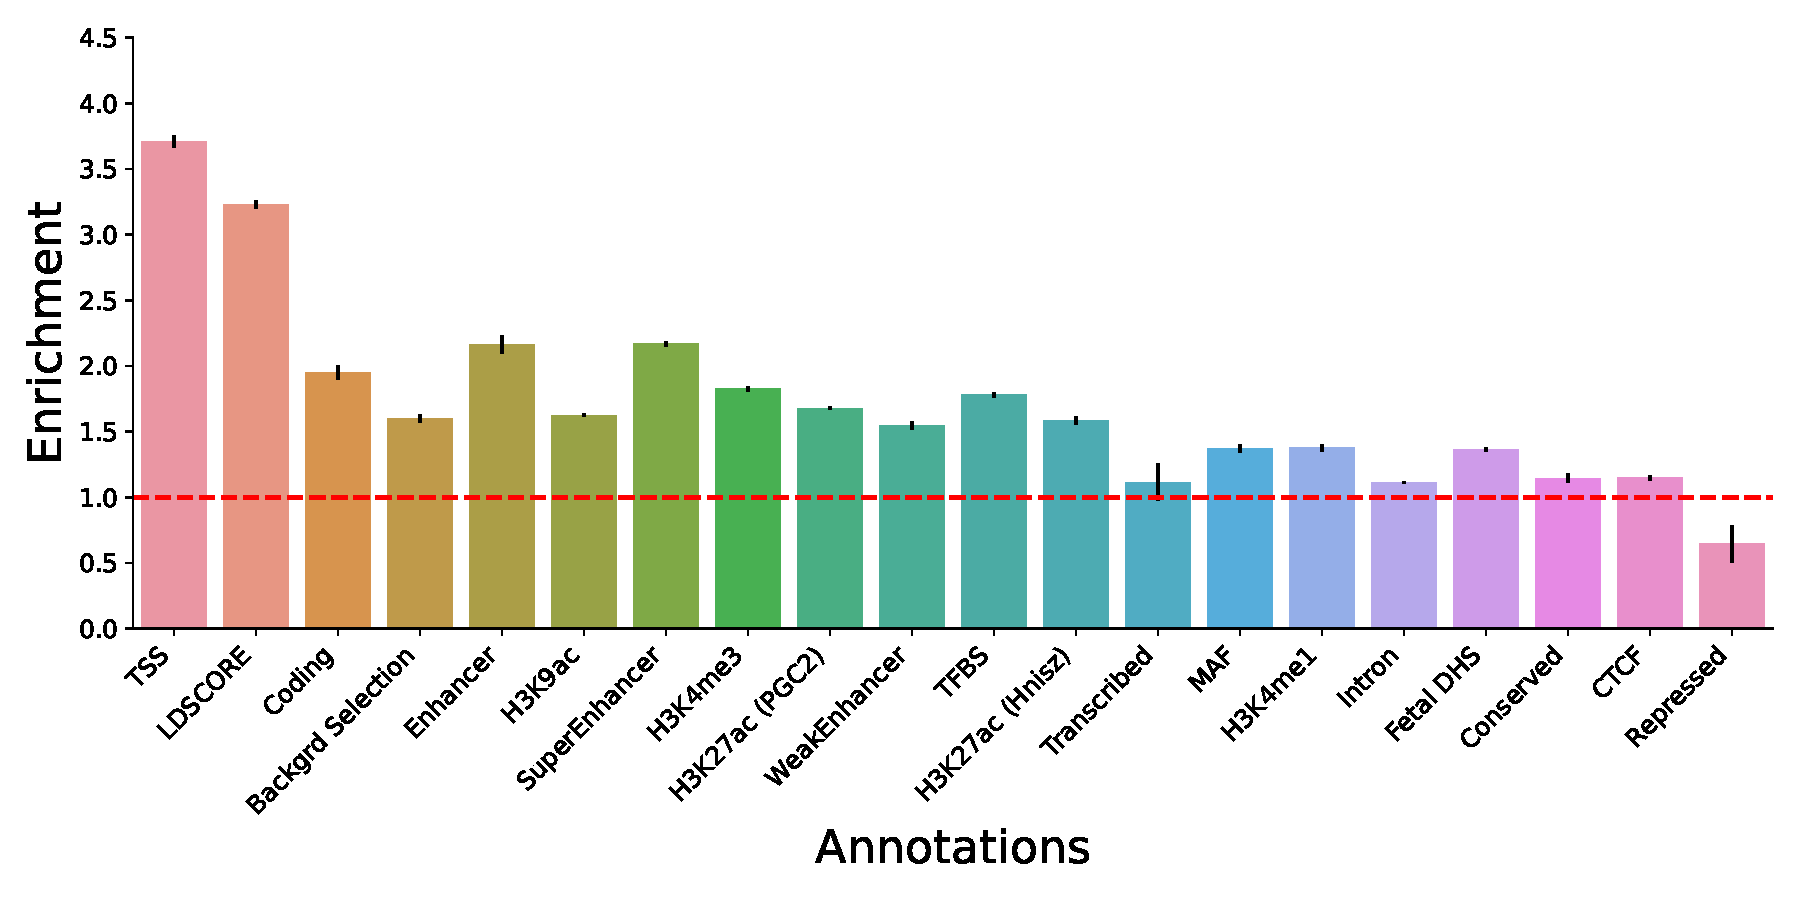
\includegraphics[width=\textwidth]{figures/functional/annotation_onlyqd_binary.pdf}
    \end{subfigure}
    \caption{\textbf{Functional enrichment at associated variants for binary traits.}
    %
    Functional enrichment profile of variants associated across $50$ binary traits.
    %
    We considered either (a) the set of variants significantly associated ($p \leq 5 \times 10^{-8}$) using both Quickdraws and REGENIE, matching the p-value distribution (see Methods), or (b) the set of variants associated using Quickdraws but not REGENIE.
    %
    Error bars represent jackknife standard errors; the red dashed line corresponds to no enrichment.
    }
    \label{fig:functional_bt}
\end{figure}

\clearpage

\subsection{Number of associations}
We assessed the number of approximately independent associations detected using each method, performing variant clumping with strict filtering criteria (p-value threshold = $5 \times 10^{-9}$, $R^2$ threshold = $0.01$).
%
A summary of these results for Quickdraws, REGENIE, and FastGWA, the most scalable methods we tested, is shown in Figure \ref{fig:ukb_indep}a; additional data is reported in tables \ref{tab:loci_qt} and \ref{tab:loci_bt}. 
%
The gains we observed in the number of detected associations were consistent with the increase in power observed in simulations: Quickdraws produced significantly more independent associations compared to REGENIE and FastGWA for quantitative and disease traits (binomial test $p < 1.9 \times 10^{-3}$) and a similar number of independent associations compared to BOLT-LMM for quantitative traits (total number of associations, Quickdraws $=26{,}236$, BOLT-LMM $=26{,}368$).
%
In more detail, for quantitative traits, Quickdraws found $4.97\%$ more independent associations compared to REGENIE and $22.71\%$ more compared to FastGWA; for disease traits, Quickdraws found on average $3.25\%$ more independent associations compared to REGENIE and $7.07\%$ compared to FastGWA.
%
The gain was higher in traits with high heritability or low polygenicity such as mean platelet volume ($8.04\%$ increase over REGENIE) and standing height ($26.1\%$ increase over REGENIE) \cite{zeng2021widespread}.
%

%
We also analyzed $250$ randomly sampled plasma-protein traits ($N \approx 43$k, see Methods), which have a less polygenic architecture than the other quantitative traits we considered \cite{sun2023plasma}.
%
In these analyses, Quickdraws found significantly more independent association signals compared to REGENIE (5.54\% more loci, $p = 6.6 \times 10^{-3}$, see Figure \ref{fig:ukb_indep}b).
%
Finally, we estimated the effective sample size, calculated as the average $\chi^2 - 1$ association statistic at variants that were found to be significantly associated (p $<5 \times 10^{-8}$) using linear regression model applied to unrelated homogeneous subset of the data \cite{yang2011genomic}.
%
We found the effective sample size estimated for Quickdraws to be $14.7\%$ higher ($p = 7.6 \times 10^{-4}$) than FastGWA and $3.4\%$ ($p = 0.197$) higher than REGENIE, while being similar to that of BOLT-LMM ($p = 0.46$) when applied to quantitative traits (see Figure \ref{fig:ukb_indep}c-d).
%

\begin{figure}[h!]
    \centering
    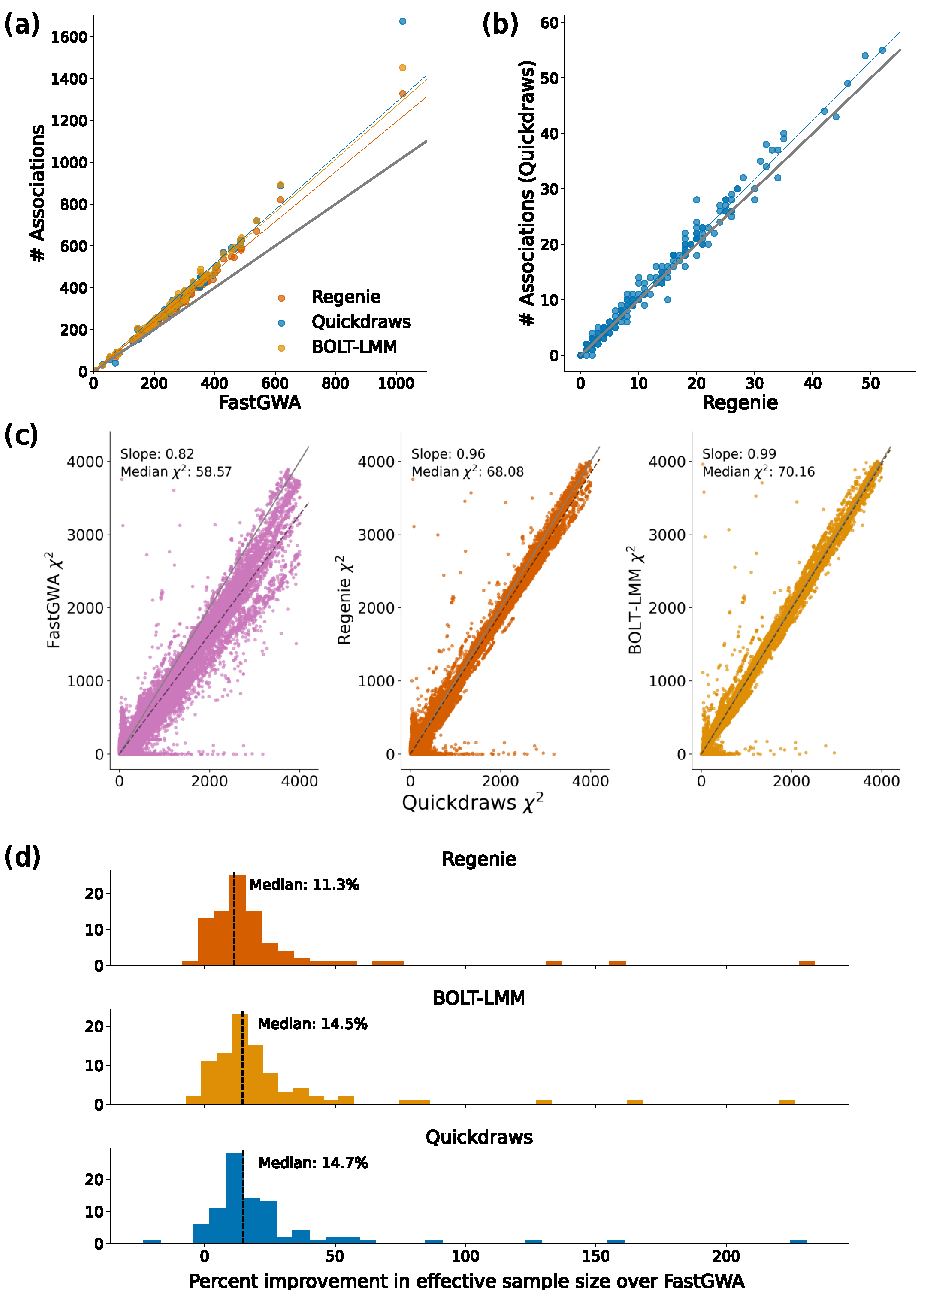
\includegraphics[scale=0.7]{figures/qd_panel_loci.pdf}
    \caption{\textbf{Approximately independent loci and effective sample size in UK Biobank analysis.} (a) Number of approximately independent loci after plink clumping in FastGWA (x-axis) vs. REGENIE, BOLT-LMM, and Quickdraws for 79 quantitative traits. (b) Number of approximately independent loci after Plink clumping in REGENIE (x-axis) vs. Quickdraws for 250 randomly sampled plasma protein traits. (c) The $\chi^2$ for 79 quantitative traits and N$=405$k UK Biobank set conditioned on genome-wide significance ($p < 5 \times 10^{-8}$) in linear regression run on unrelated subset of the data (N$=337$k). Median $\chi^2$: FastGWA $= 58.57$, REGENIE $= 68.08$, BOLT-LMM $= 70.16$, Quickdraws $= 70.64$. (d) Histogram of the effective-sample size increase compared to FastGWA for 79 quantitative traits, measured as the mean $\chi^2$ minus 1 at genome-wide significant variants inferred though linear regression run on unrelated subset of the data (N$=337$k). For (a-c) The gray line represents the y=x line and the dashed lines represent a linear regression fit for each method, for (d) the dashed line represents the median improvement in effective sample-size across traits. In (c), the slope refers to the linear regression slope of the $\chi^2$ values between each pair of methods.}
    \label{fig:ukb_indep}
\end{figure}

\clearpage

\subsection{Replication analysis with Biobank Japan, Finngen and other large-scale GWAS}

To validate the additional associations detected using Quickdraws, we performed a replication analysis using GWAS summary statistics from the Biobank Japan data set \cite{nagai2017overview}, which used BOLT-LMM-Inf and SAIGE to detect associations, FinnGen, \cite{kurki2023finngen} which used REGENIE, and other trait-specific large-scale studies \cite{jostins2012host, diabetes2012large, dubois2010multiple, nagel2018meta, de2017genome}
%
We assessed the number of variants detected using different GWAS methods that can be replicated in the Biobank Japan, FinnGen and other large-scale studies, using downloaded summary association statistics.
%
We considered $30$ quantitative traits and $13$ self-reported disease traits from Biobank Japan, as well as $21$ self-reported disease traits from FinnGen for which equivalent definitions were available in both our analyses and the replication data set, and for which at least one significant association was detected in both studies.
%
We also considered 5 disease traits (Crohn's disease \cite{jostins2012host}, Type 2 Diabetes \cite{diabetes2012large}, Celiac disease \cite{dubois2010multiple}, Depression \cite{nagel2018meta} and Ulcerative Colitis \cite{de2017genome}) that have publicly available summary statistics calculated on higher number of cases than in the UK Biobank.
%
We considered variants with MAF $\geq 0.1\%$, INFO score $\geq 0.8$, and appearing in both UK Biobank and the replicating dataset, leading to ${\sim}5.89$ million variants available for Biobank Japan replication, and ${\sim}10.89$ million variants available for FinnGen replication.
%

%
We separately considered the replication of associated variants and loci.
%
For the replication of individual variants, we assessed the number (and proportion) of variants detected ($P_{dis} \leq 5 \times 10^{-9}$) in the UK Biobank that are also significant in Biobank Japan, using multiple replication thresholds, $P_{rep} \leq 5 \times 10^{-2}$, $P_{rep} \leq 5 \times 10^{-4}$, and $P_{rep} \leq 5 \times 10^{-6}$.
%
Where, $P_{dis}$ and $P_{rep}$ are the significance thresholds for discovery and replication.
%
For the replication of loci, we followed a procedure similar to that adopted in \cite{huang2022transferability}, defining a credible set for a locus to contain a lead (or sentinel) associated variant together with additional proxy variants found within a $50$ kb window from the lead variant and with association significance $P \leq 100 \times P_{sentinel}$.
%
We defined a locus as replicated if any variant in the credible set was also found to be associated (at $P \leq 5 \times 10^{-2}$) with the same direction of effect in the replication cohort.
%
First, we calculated the average replication rate for each trait using all GWAS methods (FastGWA, REGENIE, and Quickdraws) with a discovery threshold of $5 \times 10^{-9}$.
%
Then, we adjusted the discovery threshold for each method, varying it from $2 \times 10^{-9}$ to $8 \times 10^{-9}$, to achieve the same replication rate for each method.


Across the $53$ quantitative and disease traits available in Biobank Japan and Finngen (which comprise $40$ independent traits based on squared phenotypic correlation $\leq 0.1$), Quickdraws yielded a significantly higher number of replicated loci compared to REGENIE (binomial test $p=0.014$) and FastGWA (binomial test $p=7 \times 10^{-4}$).
%
For the set of $30$ quantitative traits present in both studies, we observed a $2.5\%$ and $15.72\%$ increase over REGENIE and FastGWA, respectively, and a similar number of replicated loci compared to BOLT-LMM (total number of replicated loci, Quickdraws $=37{,}210$, BOLT-LMM $=37{,}072$).
%
For the smaller set of $23$ overlapping disease traits we analyzed, Quickdraws obtained $1.07\%$ and $3.38\%$ more replicated loci compared to REGENIE and FastGWA, respectively.
%
We observed a similar increase in the number of replicated loci for $5$ disease traits where we had access to meta-analyzed summary statistics from large-scale studies (see Table \ref{tab:repl5}).
%
We verified that this increase in the number of replicated loci did not correspond to a decrease in replication rates across these methods (see Table \ref{tab:repl1} and Figure \ref{fig:ukb_repl}d-e).
%
A Venn diagram depicting the relationships between sets of variants replicated using different methods is shown in Figure \ref{fig:ukb_repl}b-c.
%
Note that these results may be affected by the choice of GWAS method used in the replication cohort.

\begin{figure}[h!]
    \centering
    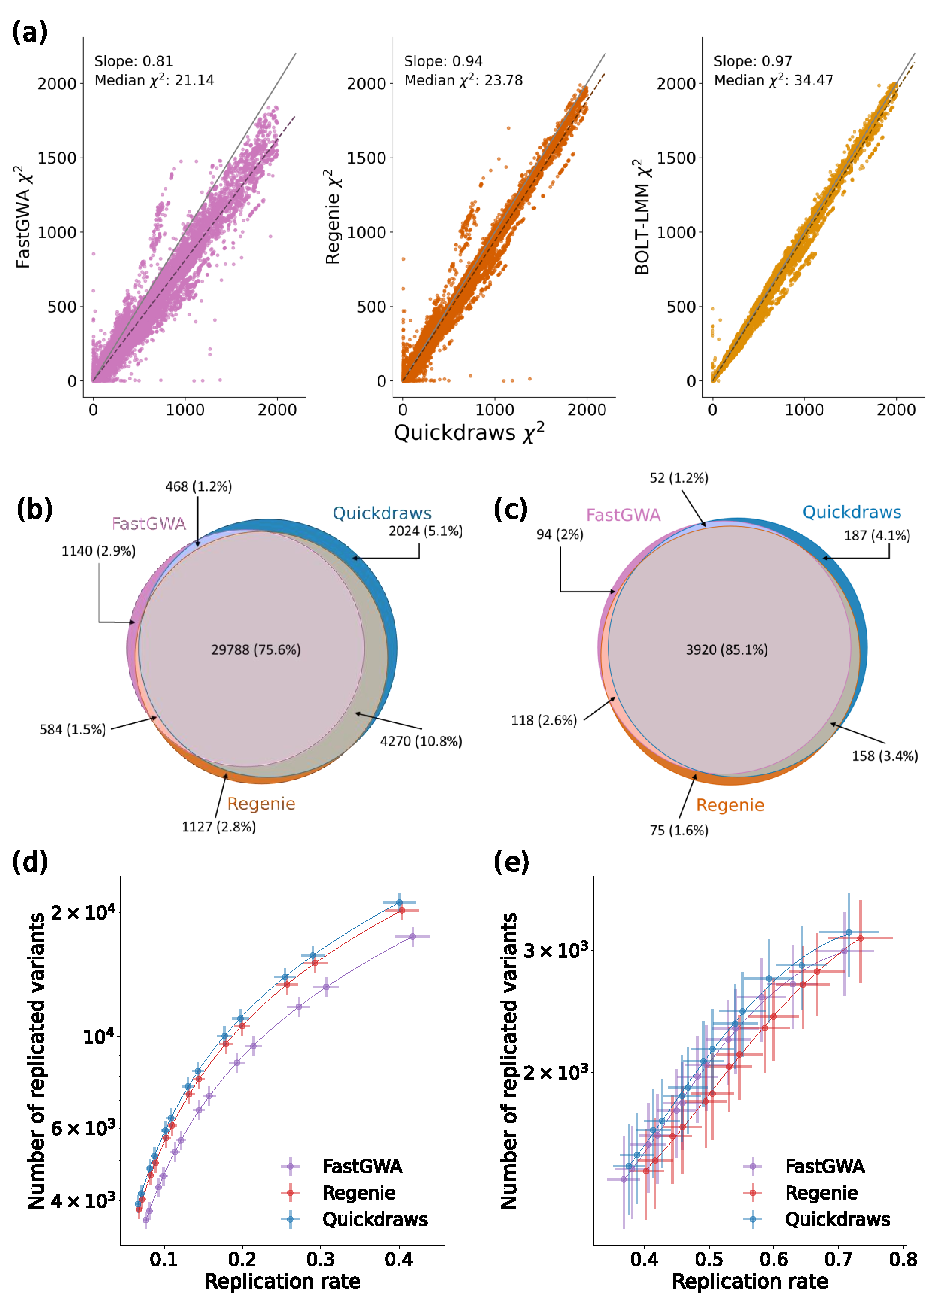
\includegraphics[scale=0.7]{figures/qd_panel_replication.pdf}
    \caption{\textbf{Replication analysis in Biobank Japan and Finngen.} (a) The $\chi^2$ in UK Biobank conditioned on genome-wide significance ($p < 5 \times 10^{-8}$) in replicating biobank across GWAS methods. The variants are aggregated across traits, quantitative and binary traits for REGENIE and FastGWA, and only quantitative traits for BOLT-LMM. The gray line represents the y=x line, and the dashed line the linear regression fit without intercept. Median $\chi^2$ for quantitative traits: FastGWA $= 28.36$, REGENIE $= 33.44$, BOLT-LMM $= 34.47$, Quickdraws $= 36.32$; binary traits: FastGWA $= 14.08$, REGENIE $= 14.34$, Quickdraws $= 14.51$. (b-c) Replication venn diagram for (b) 30 overlapping quantitative traits in Biobank Japan and (b) 23 overlapping binary traits in Biobank Japan and Finngen. (d-e) Number of replicated variants vs replication rate for (d) quantitative and (e) binary traits. The discovery threshold was fixed to $5 \times 10^{-9}$ and the replication threshold was varied from $5 \times 10^{-2}$ to $5 \times 10^{-8}$. The error bars represent standard errors calculated using block jack-knife across chromosomes. The dashed line represents a cubic spline fit to the datapoints. In (a), the slope represents the linear regression slope of the $\chi^2$ values between methods, and in (b-c), the percentages indicate the proportion of associations found with respect to the union of all methods.}
    \label{fig:ukb_repl}
\end{figure}



\clearpage

\subsection{Predictive power in out-of-sample data}
\label{sec:ch5-qd-pgs}

To verify that these power gains are due to the modeling of non-infinitesimal trait architectures, we measured the accuracy of the polygenic predictions computed by Quickdraws, BOLT-LMM, and BOLT-LMM-Inf during the model fitting step \cite{loh2015efficient,loh2018mixed}.
%
To this end, we used predictors from step 1 trained on the ${\sim}405{,}000$ white British subset to perform trait prediction for the remaining individuals.
%
Across $79$ quantitative traits, Quickdraws and BOLT-LMM obtained a mean correlation between true and predicted trait in the held-out European samples of $0.307$ (s.e $= 0.0061$) and $0.313$ (s.e $= 0.0061$), respectively, whereas BOLT-LMM-Inf yielded a lower correlation of $0.271$ (s.e $= 0.0061$) (see Figure \ref{fig:ukb_pgs}a).
%
Similar improvements due to the modeling of non-infinitesimal trait architectures have also been observed in the context of polygenic prediction \cite{vilhjalmsson2015modeling,loh2015efficient,loh2018mixed,lloyd2019improved,prive2020ldpred2}.
%

\subsubsection{Comparison with PGS methods}

We also compared the predictions from step 1 of Quickdraws with polygenic scores (PGS) built using recent methods \cite{euesden2015prsice, ge2019polygenic}.
%
To this end, we constructed PGS for all the $79$ quantitative traits analyzed, using either pruning and thresholding (P+T) as implemented in PRSice \cite{euesden2015prsice} or the PRS-CS method \cite{ge2019polygenic}.
%
We used summary statistics generated using various methods on the set of ${\sim}13.3$ million imputed variants to generate PGS for held-out individuals from European, South Asian, East Asian, and African subgroups of the UK Biobank.
%
We report the mean predictive $R^2$ and the $95\%$ confidence interval across all analyzed traits, obtained using a meta-analysis of Fisher-transformed estimated correlation coefficients.

%
We found Quickdraws' step 1 predictors to be significantly more accurate (paired t-test  $p < 5.6 \times 10^{-6}$ compared to PRS-CS and P+T) than summary-statistics derived PGS methods in the European held-out set, while achieving similar accuracy in other groups (see Figure \ref{fig:ukb_pgs}b).
%
In addition, we compared the accuracy of PGS estimates built based on summary association statistics obtained using different association algorithms.
%
Consistent with a recent analysis that did not observe higher accuracy for PGS built from summary statistics derived from non-infinitesimal modeling \cite{weissbrod2022leveraging}, we did not observe significant differences between using Quickdraws, BOLT-LMM, or REGENIE, but found PGS built using summary statistics from FastGWA to be significantly less predictive (paired t-test $p < 2.2 \times 10^{-4}$ for both PRS-CS and P+T in European and South-Asian held-out samples, see Figure \ref{fig:ukb_pgs}c-d).
%

\begin{figure}[h!]
    \centering
    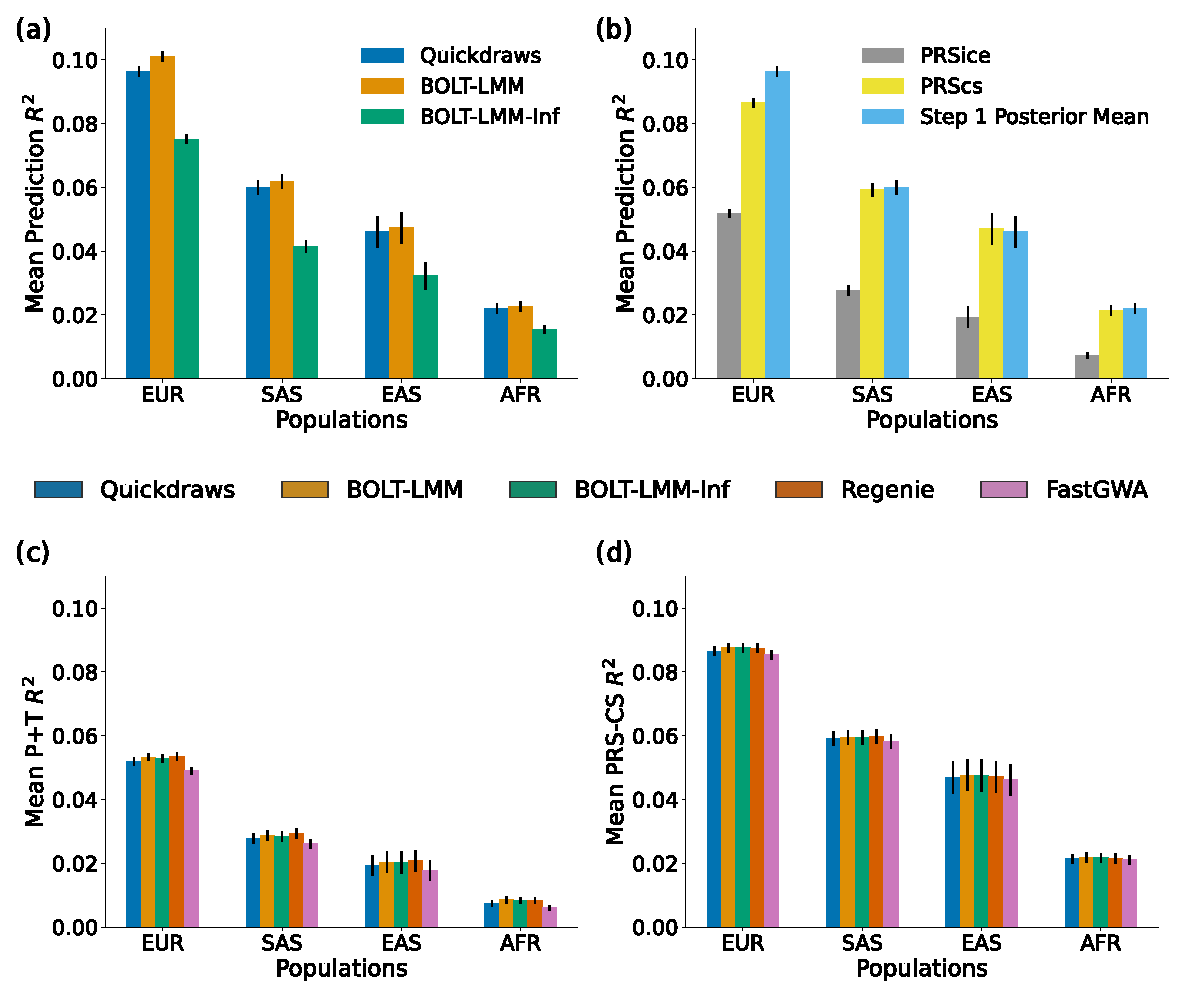
\includegraphics[width=\textwidth]{figures/qd_panel_pgs.pdf}
    \caption{\textbf{Phenotype prediction analyses in the UK Biobank.} (a) Held-out mean phenotype prediction $R^2$ comparing step 1 posterior estimates from Quickdraws, BOLT-LMM and BOLT-LMM-Inf. (b) Comparing Quickdraws' step 1 posterior estimates with PGS calculated using Quickdraws' association statistics and P+T (pruning and thresholding as implemented in PRSice) or PRS-CS. (c-d) Comparing predictive power for PGS calculated using association statistics from different GWAS methods and different PGS methods, (c) P+T as implemented in PRSice and (d) PRS-CS. All analyses was performed on $27{,}683$ held-out non-British Europeans, $9{,}044$ self-identified south Asians, $1{,}457$ self identified east Asians and $7{,}204$ self identified African of African American samples. Results are aggregated across the $79$ quantitative traits we analyzed, and the error bars represent 95\% confidence interval of the mean prediction $R^2$ for each method in each population subgroup.}
    \label{fig:ukb_pgs}
\end{figure}

\subsubsection{Comparison with PGS adjusted GWAS}

This analysis was performed by Dr. Georgios Kalantzis, who is one of the co-authors on the paper.
%
We briefly experimented with using polygenic scores as covariates when performing association, a strategy recently shown to effectively increase association power \cite{bennett2021controlling, campos2023boosting, jurgens2023adjusting}.
%
For this analysis, we focus on chromosomes $1$ to $5$, using up to $405{,}088$ samples from the white British subgroup, and analyzing all $79$ quantitative traits.
%
We first generate leave-one-chromosome-out (LOCO) polygenic scores, as described in \cite{bennett2021controlling}, using PRS-CS and summary statistics computed with FastGWA or REGENIE.
%
We then used FastGWA and REGENIE to test for association again, this time including the LOCO PGS corresponding to the chromosome of the variant being tested as a covariate, during both the model-fitting and association steps.

%
Consistent with recent results \cite{bennett2021controlling, jurgens2023adjusting}, we found that this approach increased the effective sample size for FastGWA, which relies on approximate sparse GRMs.
%
While showing no improvement in power for REGENIE, which already uses genome-wide regression to account for polygenic effects.
%
The effective sample size and total number of genome-wide significant hits, however, remained lower than that achieved using Quickdraws or BOLT-LMM (see Figure \ref{fig:prs_adjustment}).
%

\begin{figure}[h]
    \centering
    % \includegraphics[scale=0.45]{figures/fig.prs_adjustment.summary.mean_loci.chr_jknf.eps}
    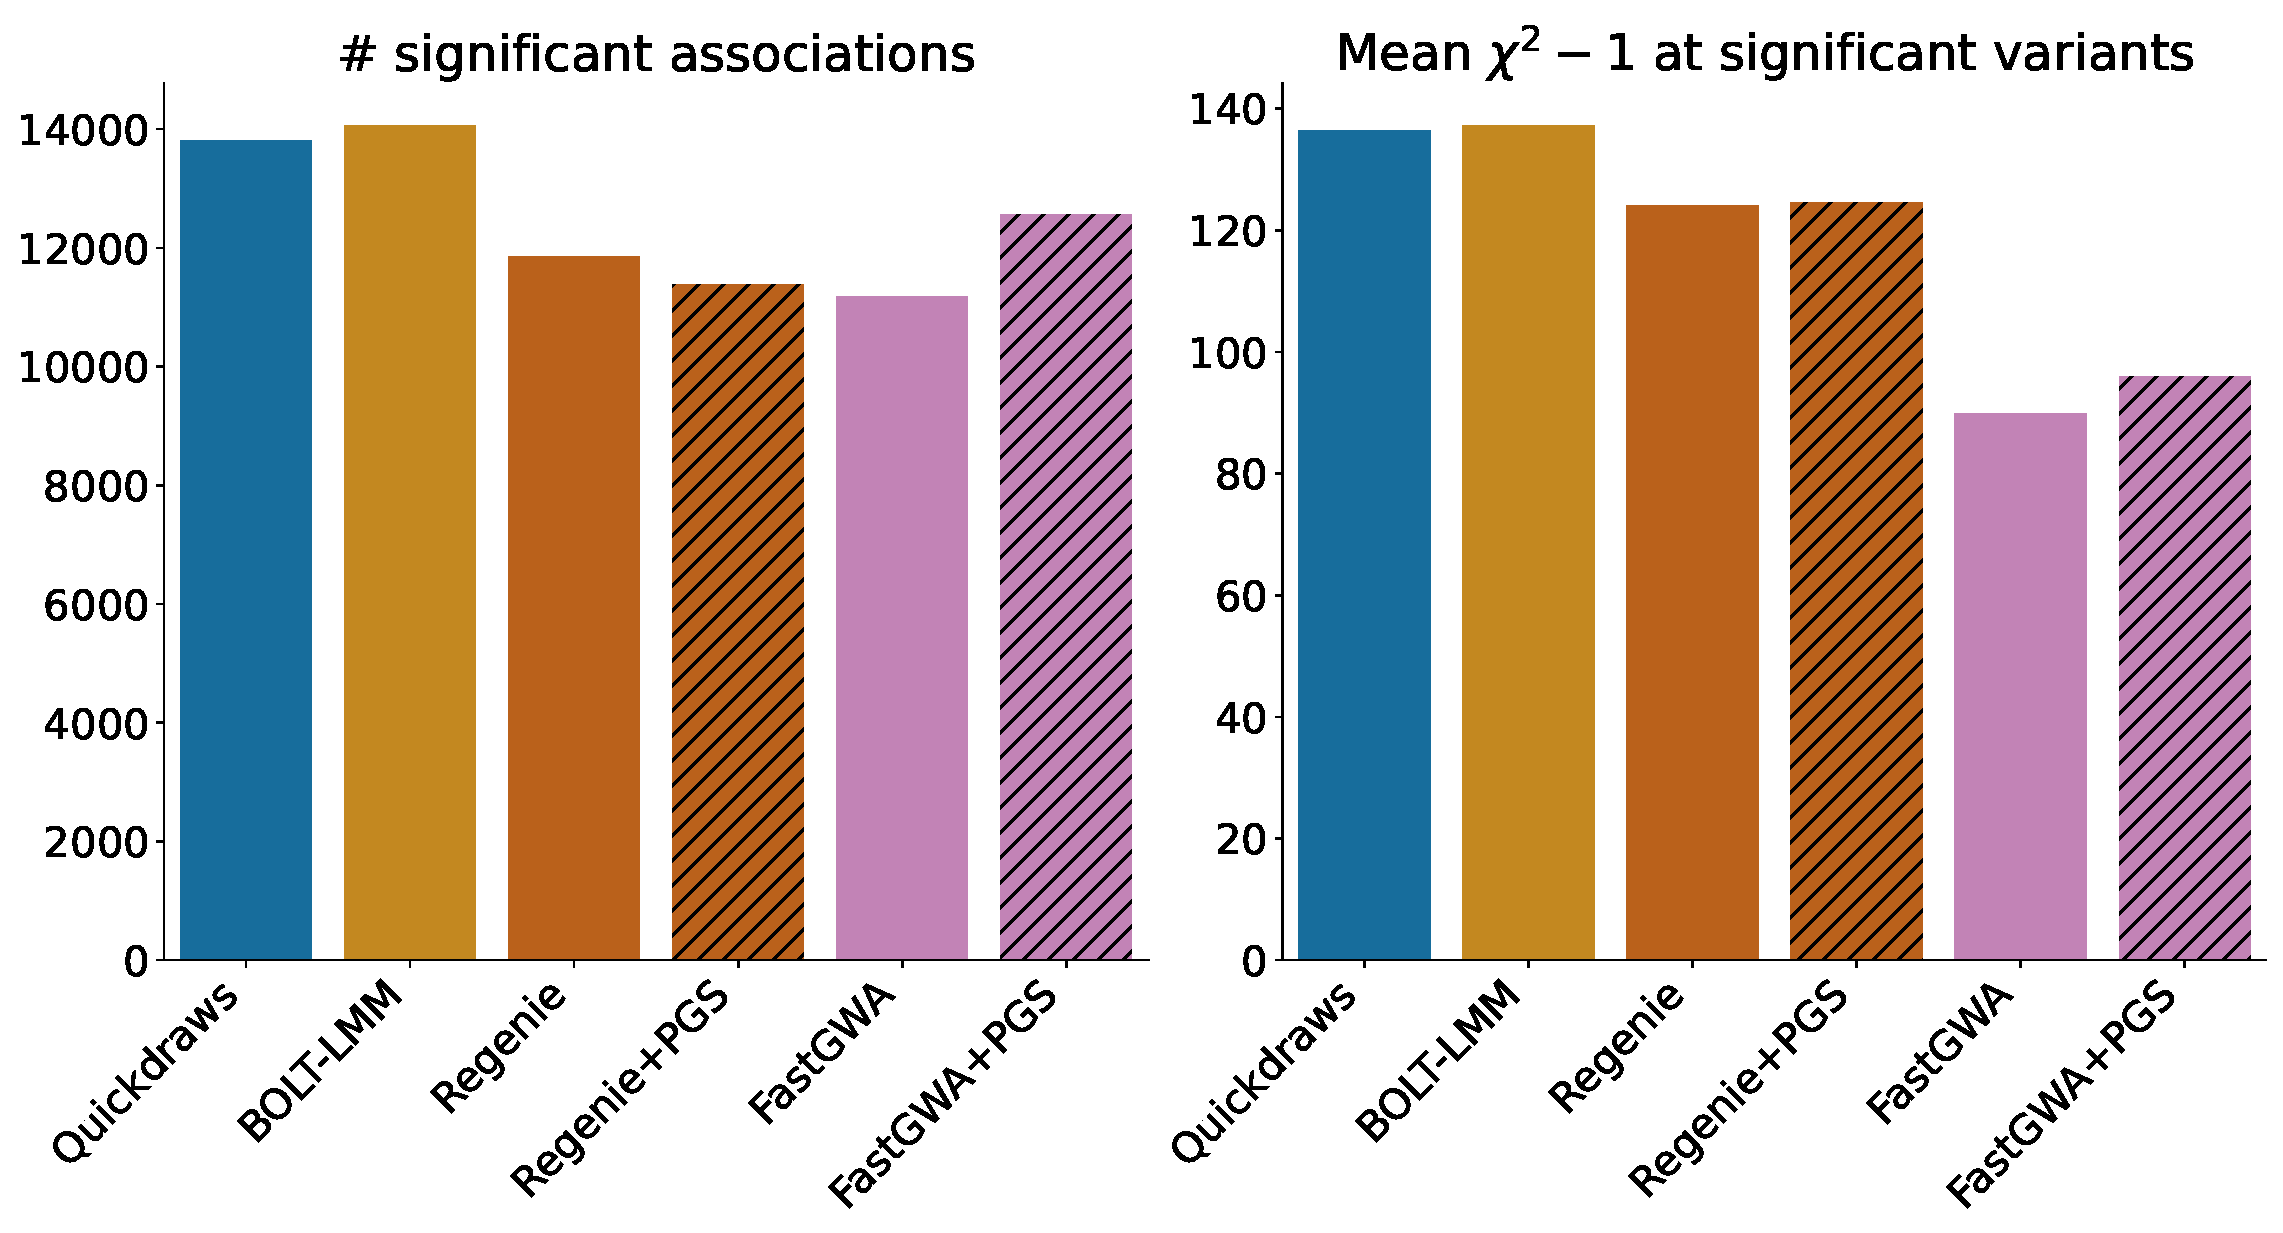
\includegraphics[width=\textwidth]{figures/fig.prs_adjustment.summary.total_loci_noCI.eps}
    % \includegraphics[scale=0.45]{figures/fig.prs_adjustment.summary.mean_loci.eps}
    \caption{\textbf{Effects of PGS-adjustment on association power.}
    %
    (a) Total number of independent loci found on chromosomes 1-5, using different GWAS methods with and without PGS adjustment in $79$ UK Biobank quantitative traits.
    %
    (b) Mean $\chi^2$ - 1 at significant variants with and without PGS adjustment for the same traits and regions.
    %
    Significant variants were defined as those with LR-unrel p-value $\leq 5 \times 10^{-8}$.
    %
    FastGWA with PGS adjustment yielded an increase in the number of independent loci (with PGS adjustment, $159.1$; without, $141.6$; paired $t$-test $p=1.9\times 10^{-9}$) and higher mean $\chi^2$-1 at significant variants (with PGS adjustment, $96.0$; without, $89.8$; $p=3.3\times 10^{-11}$).
    %
    REGENIE with PGS adjustment yielded fewer independent loci (with PGS adjustment, $144.1$; without, $150.1$; $p=7.4\times 10^{-6}$), and similar mean $\chi^2$ - 1 values (with PGS adjustment, $124.6$; without, $124.1$; $p>0.05$).
    }
    \label{fig:prs_adjustment}
\end{figure}

\clearpage

\subsection{Correction of participation bias}
\label{sec:ch5-ukb-parti-bias}

Quickdraws implements functionality to optionally correct for participation bias when computing association statistics in step 2, using an approach closely related to the one proposed in \cite{schoeler2023participation}.
%
This approach relies on the use of sampling weights, which are computed by considering a range of covariates and are used to up-weight or down-weight individuals estimated to be under-sampled or over-sampled in the study \cite{schoeler2023participation}.
%
Quickdraws takes these weights as input and performs a weighted linear regression, using a Huber-White estimator to compute the variance of the fixed effects in the regression.
%
The test statistics are recalibrated using a weighted linear regression, by matching the effective sample size estimated from a weighted linear regression on an unrelated and homogeneous sample, similar to the unweighted case.
%

%
To apply this approach in the analysis of Table \ref{tab:loci_wgwa}, we analyzed $79$ quantitative traits and $338{,}738$ individuals from the white British subgroup for which all the covariates used in \cite{schoeler2023participation} to estimate sampling weights were available.
%
These covariates included sex, age, education age, alcohol consumption frequency, smoking status, income, household size, employment status, body mass index, overall health, height, urbanization, weight, assessment center, self-reported ethnicity, and years of education.
%
We used the LASSO regression model provided in \cite{schoeler2023participation} to estimate these sampling weights and compared the number of approximately independent loci identified using LDAK with a similar participation bias adjustment but applied on unrelated homogeneous subset of the data.
%

\section{Cost analysis on UK Biobank RAP}
\label{sec:ch5-cost}

We compared the computational efficiency of Quickdraws in large-scale UK Biobank analyses to that of REGENIE, FastGWA, SAIGE, and BOLT-LMM, testing the speed and cost of running each method on the UK Biobank's RAP cloud platform.
%
We tested ${\sim}13.3$ million imputed genotypes for association with the $50$ quantitative and $50$ binary traits varying the number of samples between $N=50{,}000$, $N=405{,}088$ and artificially simulated $N=1{,}000k$.
%
We used $458{,}464$ markers for model fitting for Quickdraws, REGENIE, and BOLT-LMM and an LD-pruned set of $89{,}177$ markers for SAIGE, and used precomputed sparse GRM matrices for FastGWA and SAIGE.
%
Unlike current approaches, Quickdraws allows leveraging GPU hardware to speed up the Bayesian regression in the model fitting step.
%
To provide a more detailed overview of computational costs and to optimize the hardware configuration used for each approach, we tested all methods on up to four different RAP machines.

\sloppy
For $N = 50k$, we consider \texttt{mem3\_ssd1\_v2\_x4}, \texttt{mem2\_ssd1\_v2\_x8}, and \texttt{mem1\_ssd1\_v2\_x16}; for $N = 405k$, we consider \texttt{mem2\_ssd1\_v2\_x8}, \texttt{mem2\_ssd1\_v2\_x16}, \texttt{mem1\_ssd1\_v2\_x36}, and \texttt{mem1\_ssd1\_v2\_x72}
\sloppy
%
; for $N = 1{,}000k$, we only consider \texttt{mem1\_ssd1\_v2\_x36}.
Additionally, we use \texttt{mem2\_ssd2\_gpu1\_x8} to run step 1 of Quickdraws on an instance providing a 24GB Nvidia A10G GPU.
%
All the jobs on RAP were run using ``on-demand'' priority.
%
Each method was run using configurations that would optimize performance, where possible, example, by allowing multi-threading and supplying files using the most efficient file formats, and all methods were given the same file containing testing variants as input.

BOLT-LMM, FastGWA and SAIGE do not leverage multi-trait parallelization, so we run them for $5$ phenotypes and extrapolate the results for $50$ phenotypes.
%
We also only run BOLT-LMM for one of the three RAP instances, as the large difference in running costs would not to be significantly reduced using other types of hardware.
%
For binary traits and $N = 1{,}000k$, which are more computationally intensive, we run step 2 for Quickdraws, REGENIE, and SAIGE using a subset of ${\sim}13.3$ million testing variants, and linearly extrapolate the results.

%
Additionally, Quickdraws allows running the model-fitting step in either high-memory or low-memory mode.
%
The high-memory mode allows for loading the genotype matrix in memory for faster access.
%
The low-memory mode uses a multi-threaded approach to stream the genotype data from disk, decreasing the total memory footprint, while being marginally slower than the high-memory option ($20\%$ slower on the RAP instance we tested).
%
For the analysis in table \ref{tab:speed}, we report the minimal cost across the RAP machines we considered for each method, along with running time and total memory usage computed on a common machine, using the high-memory option for Quickdraws. A more detailed cost analysis can be found in table \ref{tab:speed_quant}, \ref{tab:speed_bin}, \ref{tab:speed_1trait} and \ref{tab:speed_1m}.

\begin{footnotesize}    
\begin{table}[h!]

    \begin{subtable}[h]{\textwidth}
    \centering
    \resizebox{\textwidth}{!}{
    \begin{tabular}{|c|c|c|c|c|c|c|}
    \hline
        Samples & Method & Step 1 & Step 2 & Total time & Total memory* & Cost on RAP** \\ 
        & & (h) & (h) & (h) & (GB) & (£) \\ \hline
        \multirow{1}{*}{50k}
            % & Quickdraws (A100) & 1.3 & 10.3 & 11.6 & 48 (16) & -\\
            & Quickdraws & 9.6 & 9 & 18.6 & 48 (16) & 7.9\\
            & BOLT-LMM & 127 & 671.5 & 798.5 & $<$15 & 158.4\\
            & REGENIE & 1.1 & 19.4 & 20.5 & $<$15 & 4.0\\
            & FastGWA & - & 20.2 & 20.2 & $<$15 & 3.6\\
        \hline    
        \multirow{1}{*}{405k}
            % & Quickdraws (A100) & 10.6 & 39.3 & 49.9 & 63 (16) & -\\
            & Quickdraws & 97.7 & 51.5 & 149.3 & 63 (16) & 93.0 \\
            & BOLT-LMM & 1,150 & 7,250 & 8,400 & 46 & 7500.0\\
            & REGENIE & 4.7 & 45.3 & 50.0 & $<$15 & 24.2\\
            & FastGWA & - & 128.4 & 128.4 & $<$15 & 37.3\\
        \hline
    \end{tabular}
    }
    \caption{Quantitative traits}
    \end{subtable}
     
     \vspace{5mm}
     
    \begin{subtable}[h]{\textwidth}
    \centering
    \resizebox{\textwidth}{!}{
    \begin{tabular}{|c|c|c|c|c|c|c|}
    \hline
        Samples & Method & Step 1 & Step 2 & Total time & Total memory* & Cost on RAP** \\ 
        & & (h) & (h) & (h) & (GB) & (£) \\ \hline
        \multirow{1}{*}{50k}
            % & Quickdraws (A100) & 1.3 & 10.3 & 11.6 & 48 (16) & -\\
            & Quickdraws & 18.3 & 77.8 & 96.1 & 49 (16) & 25.2 \\
            & SAIGE  & 2.1 & 270.9  & 273 & $<$15 & 47.5 \\
            & REGENIE  & 13.1 & 168.9 & 182.0 & $<$15 & 41.0 \\
            & FastGWA  & - & 40.6 & 40.6 & $<$15 & 9.2 \\
        \hline    
        \multirow{1}{*}{405k}
            % & Quickdraws (A100) & 10.6 & 39.3 & 49.9 & 63 (16) & -\\
            & Quickdraws  & 162.7 & 519.7 & 682.3 & 67 (16) & 395.9 \\
            & SAIGE  & 9.0 & 12015.5 & 12024.4 & $<$15 & 2834.9 \\
            & REGENIE  & 56 & 813.9 & 869.9 & $<$15 & 506.9 \\
            & FastGWA  & - & 254.1 & 254.1 & $<$15 & 98.1 \\
        \hline
    \end{tabular}
    }
    \caption{Binary traits}
    \end{subtable}
    
    \caption{\textbf{Computational efficiency of Quickdraws for (a) quantitative and (b) binary trait association.} We compare the computational requirements for recent GWAS algorithms with Quickdraws to generate summary statistics for 13.3 million variants and 50 phenotypes with either $N = 50,000$ or $N = 405,088$ and $458,464$ genotyped markers for model fitting ($89,177$ genotyped markers for SAIGE, see Methods); *Total memory includes CPU RAM memory and GPU memory, only Quickdraws requires GPU memory which is reported separately in brackets; **A more detailed cost analysis can be found in table \ref{tab:speed_quant} and \ref{tab:speed_bin} Running times are computed using the same hardware for all methods (mem2\_ssd1\_v2\_x8, with $32$ GB of RAM, $8$-core processor for $N=50k$ and mem1\_ssd1\_v2\_x36, $72$ GB of RAM, $36$-core processor for $N=405k$ datasets).
    }
    \label{tab:speed}
\end{table}
\end{footnotesize}

\section{Discussion}

To fully harness the growing volumes of genomic, phenotypic, and environmental information contained in modern biobanks, existing GWAS algorithms need to optimize a complex trade-off between cost efficiency, statistical power, and robustness.
%
We developed an algorithm for genome-wide association testing, called Quickdraws, that navigates these trade-offs by combining established GWAS paradigms, such as using mixed-effect models \cite{yu2006unified,kang2008efficient,kang2010variance,zhang2010mixed,zhou2012genome,lippert2011fast,segura2012efficient,listgarten2012improved,listgarten2013fast,loh2015efficient,loh2018mixed,jiang2019resource} to handle relatedness and population structure and the use of penalized regression \cite{firth1993bias,mbatchou2021computationally} for binary traits, with recent ideas from Bayesian machine learning, such as stochastic variational inference \cite{graves2011practical,hoffman2013stochastic}, first-order gradient optimizers \cite{robbins1951stochastic,kingma2014adam}, and transfer learning \cite{pan2009survey}.
%
In addition, Quickdraws allows leveraging GPUs, which are available in modern computing platforms and have been widely adopted in machine learning applications to parallelize computationally intensive matrix operations \cite{paszke2017automatic}.
%
Overall, this strategy allows Quickdraws to achieve higher average association power than existing methods in the analysis of binary traits, and to match the association power obtained in quantitative traits by BOLT-LMM, the only other approach that enables modeling of non-infinitesimal architectures.
%
In computational benchmarks using the UK Biobank RAP cloud platform, Quickdraws required a fraction of the computational resources used by BOLT-LMM, with costs comparable to those of scalable methods with lower average association power. 
%
Summary statistics for the traits we analyzed, which comprise $79$ quantitative traits, $50$ self-reported diseases, and $2923$ plasma protein traits, are freely available for download from \href{https://www.stats.ox.ac.uk/publication-data/sge/ppg/quickdraws/}{here}.
%

%%%%%%%%%%%%%%%%%%% Third paragraph %%%%%%%%%%%
The gains in statistical power achieved by Quickdraws are equivalent to analyzing data sets that contain larger sample sizes \cite{yang2011genomic,loh2015efficient,loh2018mixed}, with our simulations showing increases in effective sample size of over $19.2\%$ for traits linked to a few thousands of causal variants.
%
Similarly, our analyses of real traits, in which we focused on quantitative traits and diseases with high heritability and phenotyping rate, yielded more independent association signals than current scalable approaches (example, $26.1\%$ and $8.04\%$ increase over REGENIE for Height and Mean platelet volume, see tables \ref{tab:loci_qt} and \ref{tab:loci_bt}).
%
Although complex traits are known to be highly polygenic \cite{yengo2022saturated}, their genetic architectures, in particular for molecular traits such as metabolites \cite{kettunen2012genome}, are estimated to be far from a purely infinitesimal model, with large fractions of heritability concentrating in a relatively small set of variants \cite{stahl2012bayesian,zeng2018signatures,weissbrod2020functionally}.
%
As the range of phenotypic measurements available in biobank data sets continues to grow, we therefore expect the increase in computational power that we observed in our analyses to also be observed in broader sets of traits and diseases.
%

\subsection{Sharing and combining posterior effect estimates}

Our analyses demonstrate that, in addition to increasing association power by allowing the computation of a residualized phenotype, the posterior mean estimates of the effect sizes computed during the model fitting step can be used to construct polygenic scores that perform well in held-out individuals compared to those computed from summary association statistics.
%
Therefore, sharing these effect estimates, which we make available for the traits we analyzed (see \href{https://www.stats.ox.ac.uk/publication-data/sge/ppg/quickdraws/}{here}), may facilitate novel downstream analyses.
%
However, compared to the use of summary association statistics, one disadvantage of using posterior effect estimates to construct polygenic scores is the lack of established methodology to combine them across independent cohorts.
%
Developing strategies that allow to meta-analyze these effects across cohorts could open new avenues for the development of federated association and polygenic prediction strategies that preserve high statistical power without the need for sharing individual-level data.
%

% mention federated learning angle, cite two bonnie berger papers 

\subsection{Limitations and future work}

We highlight several current limitations and areas of future work to improve the Quickdraws algorithm.
%
First, Quickdraws leverages modern GPU hardware to speed up the Bayesian regression in the model fitting step and is therefore slower when run on traditional CPU hardware (see Figure \ref{fig:step1_cpu_gpu} for a comparison).
%
GPUs may not be as easily accessible as CPUs, and have higher costs, as evidenced in Table \ref{tab:speed_quant} and \ref{tab:speed_bin}.
%
Our analyses on the RAP cloud platform, however, demonstrates that the overall increase in running costs is not substantial.
%
Furthermore, the extensive use of GPUs in machine learning applications is likely to continue to increase their availability, paving the way for additional GPU-based applications in human genetics.
%
Future work may allow developing a faster CPU-based implementation of Quickdraws.
%
Second, although Quickdraws is well parallelized for the analysis of multiple traits, it currently does not capture the correlations that often exist across these traits.
%
Extending Quickdraws to leverage genetic and environmental correlations is likely to lead to improved performance \cite{korte2012mixed,zhou2014efficient}.
%
%
Third, although we have shown that a strategy based on adjusting for polygenic scores computed within the same sample does not lead to power gains comparable to those achieved by Quickdraws and BOLT-LMM, it is possible that using polygenic scores constructed from larger external cohorts will lead to more substantial power increases \cite{campos2023boosting, jurgens2023adjusting}.
%
Fourth, association analyses have recently been shown to be affected by participation biases \cite{pirastu2021genetic, benonisdottir2023studying}, to which Quickdraws is also susceptible.
%
To mitigate these biases, we implemented the adjustment strategy proposed in \cite{schoeler2023participation} in step 2 of the Quickdraws algorithm (as described in Section \ref{sec:ch5-ukb-parti-bias}).
%
However, further work will be needed to incorporate this adjustment in step 1 of the algorithm.
%
Despite these current limitations and avenues for future development, we believe that Quickdraws will provide a useful tool for large-scale GWAS, demonstrating the promise of leveraging modern machine learning methodology to improve statistical power and efficiency in these analyses.

\begin{figure}
    \centering
    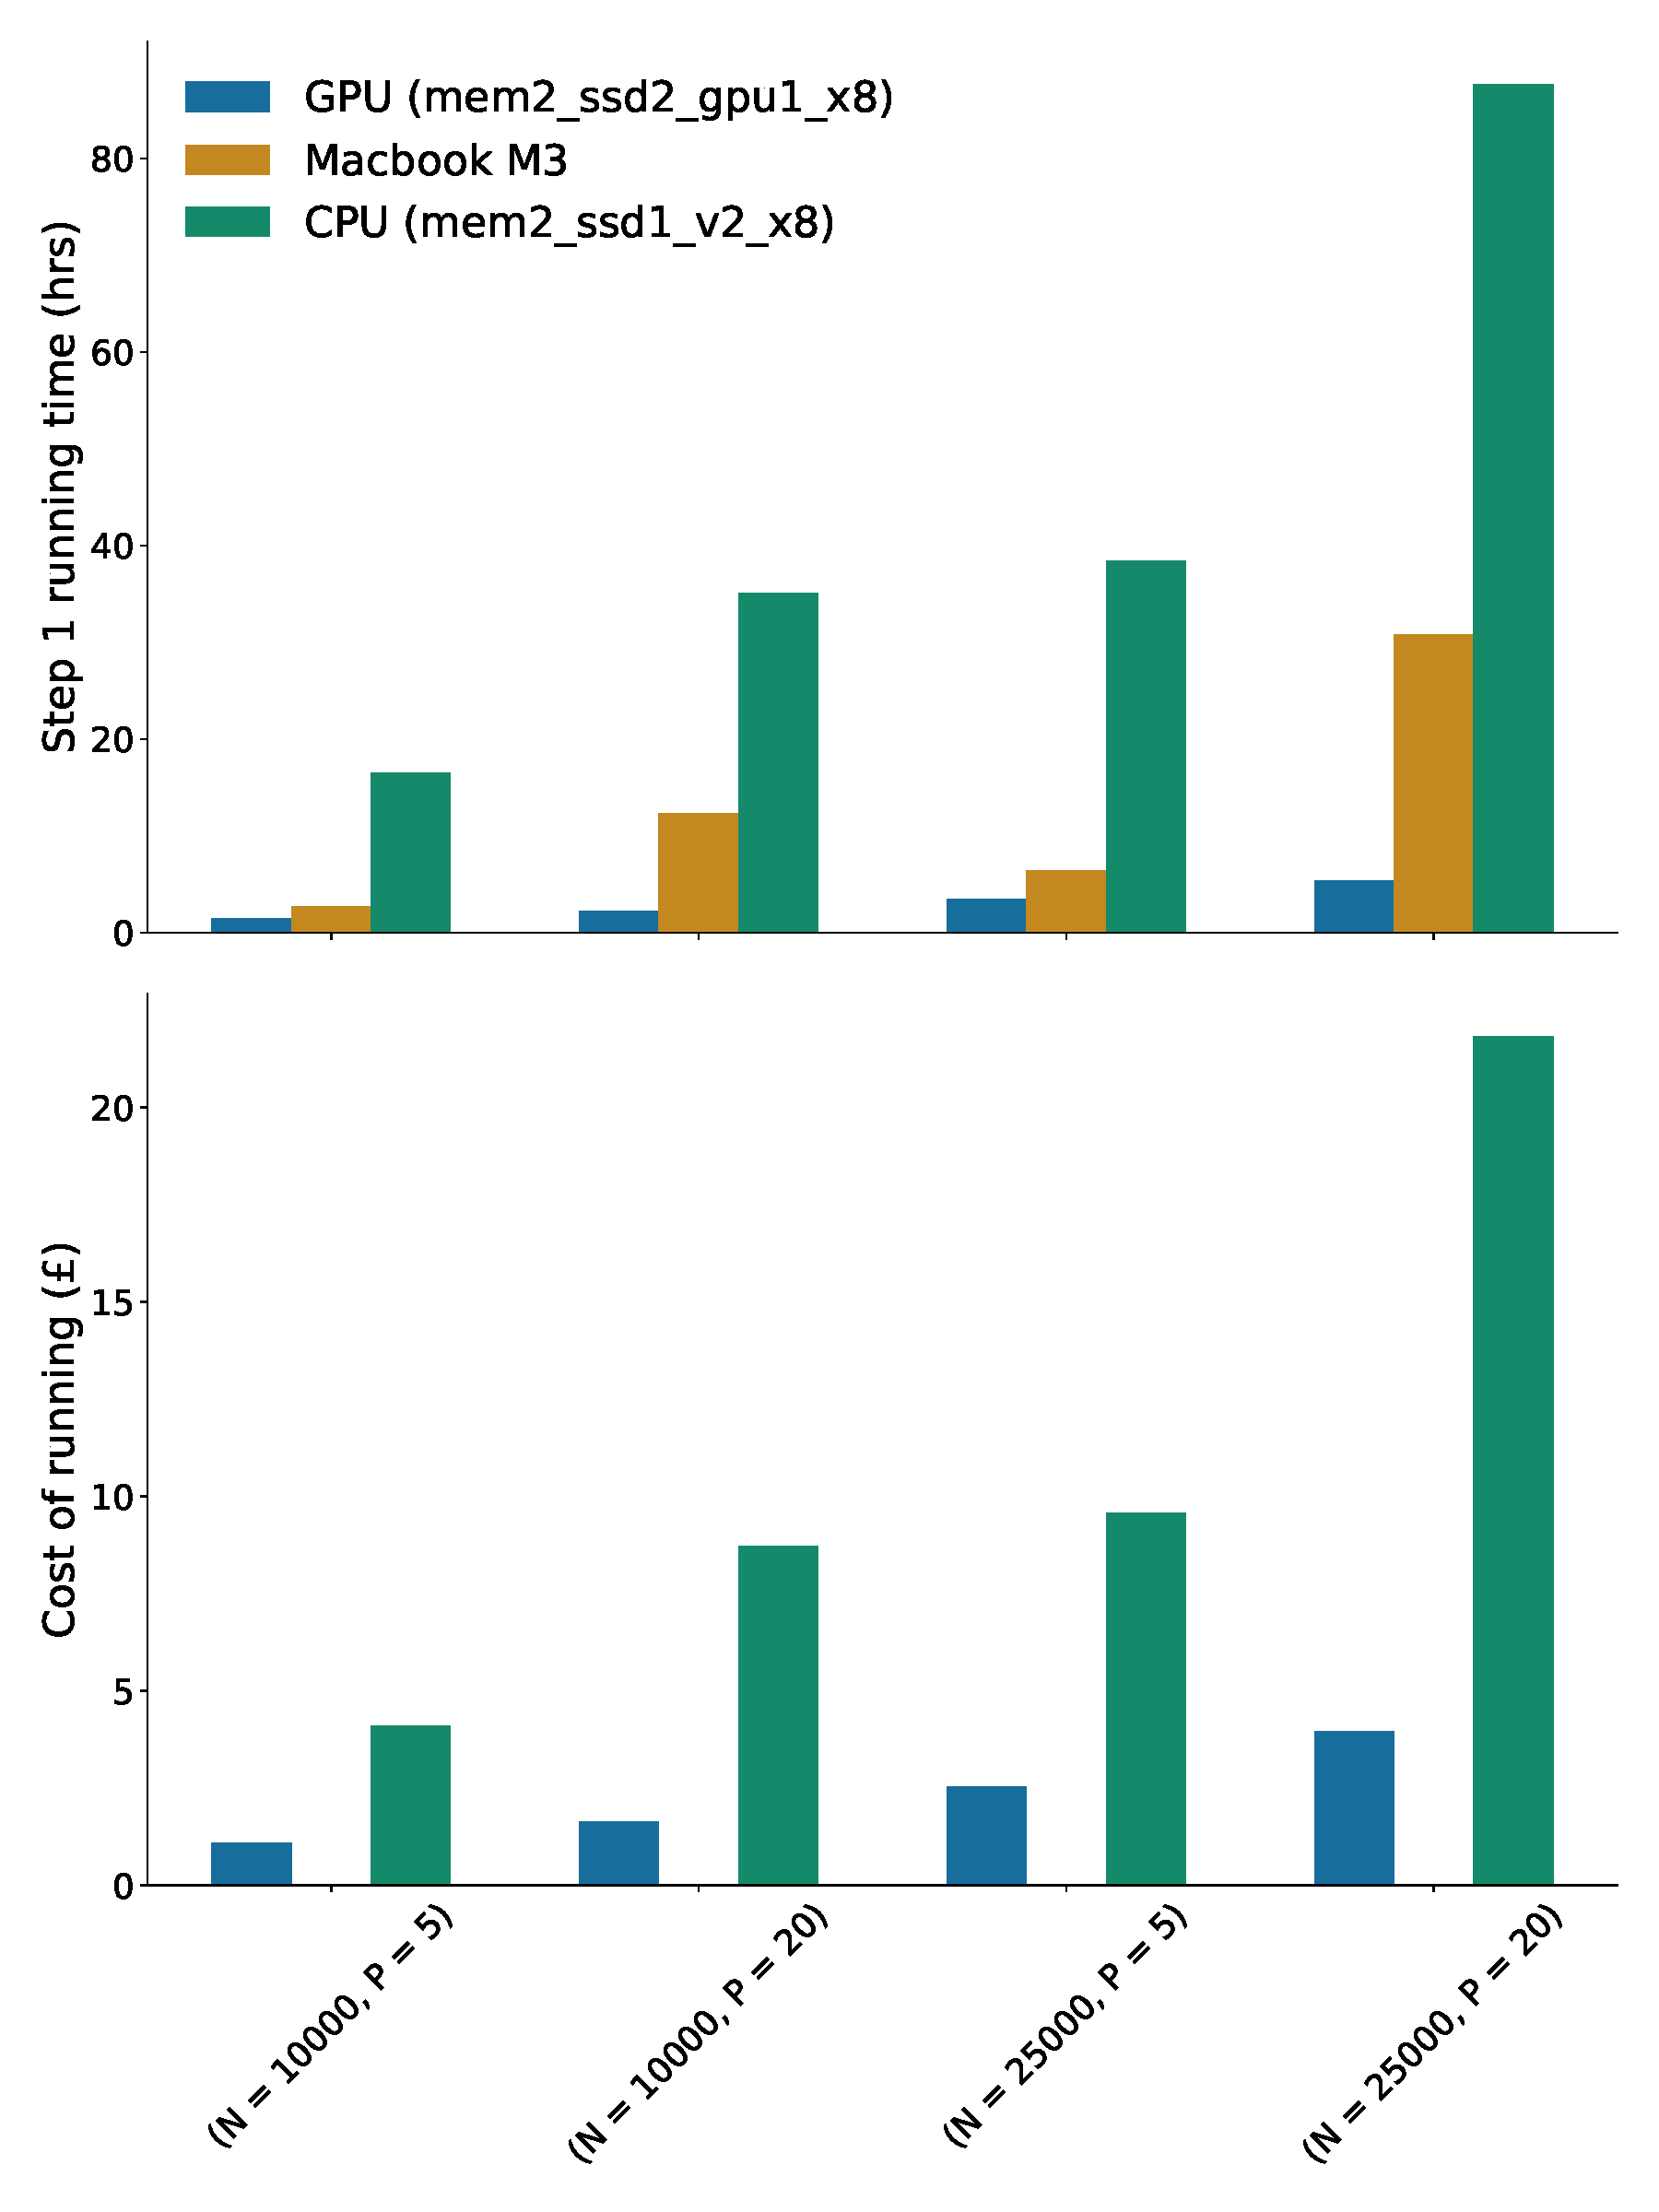
\includegraphics[width=0.75\textwidth]{figures/step1_running_time_cost.pdf}
    \caption{\textbf{Computational performance of Quickdraws on different computing architectures.} We assessed the running time and cost associated with Quickdraws' model fitting step (Step 1) across varying numbers of samples ($N$) and phenotypes ($P$). Performance was compared for three architectures: an Nvidia A10G GPU node on the UK Biobank Research Analysis Platform (RAP) (\texttt{mem2\_ssd2\_gpu1\_x8}), a 14-core MacBook Pro equipped with the Apple M3 chip, and an 8-core CPU node on the UK Biobank RAP (\texttt{mem2\_ssd1\_v2\_x8}). Running costs were calculated only for the GPU and CPU nodes on the RAP.}
    \label{fig:cpu_vs_gpu_vs_mac}
\label{fig:step1_cpu_gpu}
\end{figure}